% ===========================================================
%  Regulación del Alquiler y Dinámica del Mercado Residencial
%  en Barcelona (2000–2025)  ·  Version 2
%  Compilar con pdfLaTeX en Overleaf (dos pasadas)
% ===========================================================
\documentclass[10pt,a4paper,twocolumn]{article}

% ── Encoding & idioma ──────────────────────────────────────
\usepackage[utf8]{inputenc}
\usepackage[T1]{fontenc}
\usepackage[spanish,english]{babel}

% ── Márgenes ───────────────────────────────────────────────
\usepackage[top=2.0cm,bottom=2.0cm,left=1.6cm,right=1.6cm,
            columnsep=0.6cm]{geometry}

% ── Tipografía ─────────────────────────────────────────────
\usepackage{microtype}
\usepackage{lmodern}
\usepackage{times}

% ── Matemáticas ────────────────────────────────────────────
\usepackage{amsmath,amssymb,amsthm}
\usepackage{bm}

% ── Tablas ─────────────────────────────────────────────────
\usepackage{booktabs}
\usepackage{threeparttable}
\usepackage{multirow}
\usepackage{array}

% ── Figuras ────────────────────────────────────────────────
\usepackage{graphicx}
\usepackage{subcaption}
\usepackage{float}
\usepackage[dvipsnames]{xcolor}

% ── Hipervínculos ──────────────────────────────────────────
\usepackage[colorlinks=true,linkcolor=NavyBlue,
            citecolor=NavyBlue,urlcolor=NavyBlue]{hyperref}
\usepackage{natbib}

% ── Espaciado ──────────────────────────────────────────────
\usepackage{setspace}
\setstretch{1.05}
\usepackage{parskip}
\setlength{\parskip}{3pt}

% ── Secciones compactas ────────────────────────────────────
\usepackage{titlesec}
\titlespacing*{\section}{0pt}{8pt}{4pt}
\titlespacing*{\subsection}{0pt}{6pt}{2pt}
\titlespacing*{\subsubsection}{0pt}{4pt}{2pt}
\titleformat{\section}{\normalfont\large\bfseries}{\thesection.}{0.5em}{}
\titleformat{\subsection}{\normalfont\normalsize\bfseries}{\thesubsection.}{0.4em}{}
\titleformat{\subsubsection}{\normalfont\small\bfseries\itshape}{\thesubsubsection.}{0.4em}{}

% ── Captions ───────────────────────────────────────────────
\usepackage{caption}
\captionsetup{font=small,labelfont=bf,skip=4pt}

% ── Cabeceras ──────────────────────────────────────────────
\usepackage{fancyhdr}
\pagestyle{fancy}
\fancyhf{}
\fancyhead[L]{\small\textit{Soto et al.\ · Regulación del alquiler en Barcelona}}
\fancyhead[R]{\small\textit{2026}}
\fancyfoot[C]{\small\thepage}
\renewcommand{\headrulewidth}{0.4pt}

% ── Columna única para título / abstract ───────────────────
\usepackage{multicol}

% ── Otros ──────────────────────────────────────────────────
\usepackage{url}
\usepackage{enumitem}
\setlist[itemize]{itemsep=1pt,topsep=2pt}
\setlist[enumerate]{itemsep=1pt,topsep=2pt}

% ── Comandos propios ───────────────────────────────────────
\newcommand{\pval}[1]{$p{=}#1$}
\newcommand{\coef}[1]{$\hat{\beta}{=}#1$}
\newcommand{\MAPE}{\text{MAPE}}
\newcommand{\RMSE}{\text{RMSE}}

% ===========================================================
\begin{document}
\selectlanguage{spanish}

% ── CABECERA EN COLUMNA ÚNICA ───────────────────────────────
\twocolumn[{%
\begin{@twocolumnfalse}

\begin{center}
  {\LARGE\bfseries
   Regulación del Alquiler y Dinámica del Mercado\\[4pt]
   Residencial en Barcelona (2000--2025):\\[4pt]
   Un Análisis Multimétodo con Panel de Datos,\\[4pt]
   Clasificación Supervisada y Series Temporales}

  \vspace{8pt}

  {\large
   Katherine Soto \quad $\cdot$ \quad Juan R.\ Ortiz \quad $\cdot$ \quad Emilio Delgado}

  \vspace{3pt}
  {\normalsize La Salle -- Universitat Ramon Llull, Barcelona \quad
   $\{$\texttt{kthsoto, jrortiz, edelgado}$\}$@salleurl.edu}

  \vspace{3pt}
  {\small Proyecto 2.1 · Mini-TFM · Máster en Inteligencia Artificial y Ciencia de Datos · Abril 2026}
\end{center}

\vspace{6pt}

% Abstract en español
\begin{abstract}
\noindent
Presentamos un análisis cuantitativo del mercado de alquiler residencial de Barcelona
durante el período 2000--2025 (103 trimestres), caracterizado por tres ciclos regulatorios
sucesivos: Ley 11/2020, derogación del Tribunal Constitucional (2022) y Ley 12/2023.
Empleamos cuatro métodos complementarios sobre datos oficiales de 10~distritos y
66~barrios: \textit{(i)}~regresión de panel con efectos fijos (\textit{within}, $N{=}2.838$
observaciones barrio-trimestre); \textit{(ii)}~clasificación supervisada de episodios
de tensión contractual (Random Forest, Gradient Boosting y Regresión Logística);
\textit{(iii)}~modelos SARIMAX$(1,1,1)(1,0,1)_4$ con análisis de intervención ITS-3
sobre 30 combinaciones distrito$\times$métrica; y \textit{(iv)}~los mismos modelos
sobre la serie ciudad en tres métricas: precio nominal, precio real (base~2025) y
volumen de contratos. El ITS-3 revela que la Ley~12/2023 produce una caída estructural
en contratos ($\hat{\beta}_{D_{12}}{=}{-}1.588$, $p{=}0.007$) y un incremento
paradójico del precio real ($+0.495$\,\euro/m$^2$, $p{=}0.034$), coherente con
el efecto composición documentado en la literatura internacional. El SARIMAX alcanza
un MAPE del $3.3\,\%$ en precio nominal ciudad.
\end{abstract}

\vspace{4pt}
\noindent\textbf{Palabras clave:} regulación del alquiler · ITS multi-ruptura · panel efectos fijos · SARIMAX · tensión contractual · zona tensionada · efecto composición · Barcelona.

\vspace{8pt}

% Abstract en inglés
\begin{otherlanguage}{english}
\begin{abstract}
\noindent
We present a quantitative study of Barcelona's residential rental market over the
period 2000--2025 (103 quarters), covering three successive regulatory cycles: Law
11/2020, a Constitutional Court ruling (2022), and Law 12/2023. Four complementary
methods are applied to official quarterly data for 10 districts and 66 neighbourhoods:
\textit{(i)}~fixed-effects panel regression (\textit{within} estimator, $N{=}2{,}838$);
\textit{(ii)}~supervised classification of contractual tension episodes; \textit{(iii)}~SARIMAX$(1,1,1)(1,0,1)_4$ models with multi-break interrupted time series (ITS-3)
analysis across 30 district$\times$metric combinations; and \textit{(iv)}~the same
models on the city-aggregate series for three metrics: nominal price, real price (2025
base), and contract volume. The ITS-3 shows that Law 12/2023 causes a structural drop
in contracts ($\hat{\beta}{=}{-}1{,}588$, $p{=}0.007$) and a paradoxical real-price
increase ($+0.495$\,\euro/m$^2$, $p{=}0.034$), consistent with a composition effect.
The SARIMAX achieves 3.3\,\% MAPE on the city-level nominal price.\\[2pt]
\textbf{Keywords:} rent control · interrupted time series · fixed-effects panel · SARIMAX · contractual tension · Barcelona.
\end{abstract}
\end{otherlanguage}

\vspace{10pt}
\hrule
\vspace{8pt}
\end{@twocolumnfalse}
}]

% ===========================================================
\section{Introducción}
\label{sec:intro}

El acceso a la vivienda se ha convertido en uno de los principales retos de política
pública en las ciudades europeas del siglo~XXI. Barcelona ofrece un caso de estudio
excepcional: en el período 2020--2025 fue escenario de tres ciclos regulatorios
consecutivos --- regulación, derogación y re-regulación --- con la densidad temporal
y la desagregación geográfica suficientes para emplear métodos econométricos robustos.

La pregunta central que articula el análisis es: \textit{¿Ha modificado la regulación
del alquiler la dinámica de precios y del volumen contractual de forma estructural,
diferenciada por distrito y métrica de mercado?} La respuesta exige ir más allá de
la comparación de medias: los precios y los contratos pueden responder en sentidos
opuestos a la misma intervención, y la heterogeneidad geográfica puede ocultar efectos
cualitativamente distintos entre barrios.

\textbf{Aportación principal.} Frente a los análisis disponibles para España
\citep{garcia2018housing,bosch2021ley11}, este trabajo contribuye con: \textit{(a)}~un
horizonte de 25 años con datos trimestrales desagregados a nivel barrio y distrito;
\textit{(b)}~tres métricas simultáneas del mercado (precio nominal, precio real
deflactado, volumen contractual); \textit{(c)}~un diseño ITS con tres rupturas que
permite atribuir efectos a cada régimen de forma separada; y \textit{(d)}~30 modelos
SARIMAX a nivel distrito, lo que posibilita una comparativa de heterogeneidad
geográfica inédita en la literatura española sobre regulación del alquiler.

El artículo se organiza como sigue. La Sección~\ref{sec:relacionados} revisa la
literatura. La Sección~\ref{sec:datos} describe los datos y el pipeline. La
Sección~\ref{sec:metodos} desarrolla los cuatro módulos metodológicos. La
Sección~\ref{sec:resultados} presenta los resultados. La
Sección~\ref{sec:discusion} abre la discusión cualitativa, y la
Sección~\ref{sec:conclusiones} cierra con conclusiones y líneas abiertas.

% ===========================================================
\section{Trabajo Relacionado}
\label{sec:relacionados}

\subsection{Efectos de la regulación del alquiler}

El control de rentas es objeto de un debate económico de largo recorrido. Los modelos
de primera generación \citep{arnott1995rent} predicen que cualquier tope de precio
por debajo del equilibrio reduce la oferta en el largo plazo y deteriora la calidad
del parque. \citet{diamond2019rent} ofrecen la evidencia causal más rigurosa en
contexto moderno: explotando la ampliación del control de rentas en San Francisco como
experimento natural, documentan una caída del $15\,\%$ en la oferta de viviendas
reguladas con reconversión hacia usos alternativos, y un incremento de precios del
$5$--$7\,\%$ en el segmento no regulado adyacente. \citet{sims2007rent} llega a
conclusiones similares con la desregulación de Massachusetts: la eliminación del
control eleva la oferta de forma significativa.

Para Europa, \citet{kholodilin2021rent} analiza la \textit{Mietendeckel} de Berlín
(2020--2021) con un diseño de diferencias en diferencias y documenta una reducción del
precio en el segmento regulado acompañada de una contracción paralela de la oferta
observable, patrón consistente con los hallazgos que presentamos para Barcelona.

\subsection{Métodos cuantitativos en análisis de políticas}

El diseño de series temporales interrumpidas \citep{wagner2002its} es el estándar
metodológico para la evaluación de intervenciones de política cuando el grupo de
control no existe o no es comparable. \citet{angrist2009mostly} sitúan el ITS como
un caso particular de regresión de discontinuidad en el tiempo: la identificación
descansa en la discontinuidad del sendero temporal en la fecha de intervención.
\citet{baltagi2021econometric} fundamenta el estimador \textit{within} para datos de
panel con efectos fijos, que elimina toda heterogeneidad barrio-específica fija y
concentra la identificación en la variación temporal dentro de cada unidad.

Para la parte predictiva, \citet{hyndman2021forecasting} recomienda validar siempre
contra el naïve estacional antes de aceptar modelos más complejos; la especificación
SARIMAX sigue a \citet{box2015timeseries}. En clasificación, el protocolo de
validación cruzada temporal con \texttt{TimeSeriesSplit} es el estándar para evitar
\textit{data leakage} en series con estructura temporal \citep{bergmeir2018note}.

% ===========================================================
\section{Datos y Preparación}
\label{sec:datos}

\subsection{Fuente y cobertura}

Los datos provienen del Portal de Dades Obertes del Ajuntament de Barcelona, dataset
\textit{Contractes de lloguer per districtes i barris} (actualización trimestral).
La cobertura es 2000Q1--2025Q3 ($T{=}103$ trimestres), con información para
10~distritos y 73~barrios, de los cuales se excluyen 7 de mercado delgado (mediana
inferior a 300 contratos/trimestre) para garantizar robustez estadística. Variables
macroeconómicas adicionales (IPC, Euríbor 12m) se incorporan mediante \textit{merge}
temporal desde el INE y el Banco de España.

\subsection{Variables analíticas}

Definimos tres métricas de análisis que cubren dimensiones complementarias del mercado:

\vspace{2pt}
\noindent\textbf{Precio nominal:}
$\texttt{avg\_rent\_m2}_t = \frac{\sum_i w_{it}\,r_{it}}{\sum_i w_{it}}$,
donde $r_{it}$ es la renta media por m$^2$ del distrito $i$ y $w_{it}$ es el número
de contratos. Esta media ponderada elimina el sesgo de composición de tamaño de distrito.

\noindent\textbf{Precio real:} $\texttt{avg\_rent\_m2\_real}_{t} =
\texttt{avg\_rent\_m2}_t \times \frac{100}{\text{IPC}_t^{(2025)}}$,
deflactado con el IPC (base~2025), disponible desde 2002Q1.

\noindent\textbf{Volumen:} $\texttt{num\_contracts}_t = \sum_i n_{it}$,
suma total de contratos registrados en el trimestre.

\subsection{Pipeline de limpieza}

La Figura~\ref{fig:eda_series} muestra la evolución de las tres métricas para
Barcelona agregado.

\begin{figure}[H]
  \centering
  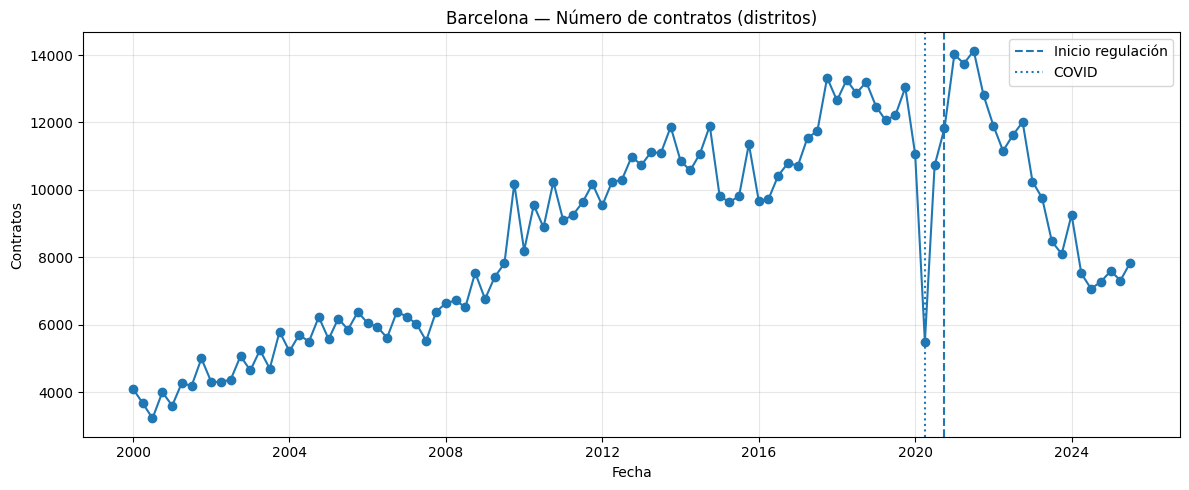
\includegraphics[width=\linewidth]{figures/fig_eda_series.png}
  \caption{Series trimestrales de Barcelona (2000--2025). Las líneas verticales
    señalan COVID (gris punteado) y regulación 2020Q4 (rojo discontinuo).}
  \label{fig:eda_series}
\end{figure}

El precio nominal creció de 6.01~\euro/m$^2$ (2000) a 16.85~\euro/m$^2$ (2025),
un incremento del $+180\,\%$ nominal pero solo $+14\,\%$ en términos reales.
La construcción del índice temporal completo se realiza con
$\texttt{pd.date\_range(freq='QS-OCT')}$ e interpolación temporal lineal para huecos
internos; el tratamiento se aplica a nivel barrio antes de agregar para no propagar
artefactos numéricos al nivel ciudad.

\subsection{Análisis exploratorio y cambio estructural}

La Figura~\ref{fig:eda_5periods} desglosa las distribuciones por los cinco períodos
regulatorios. La Tabla~\ref{tab:prepost} reporta los tests estadísticos formales.

\begin{figure}[H]
  \centering
  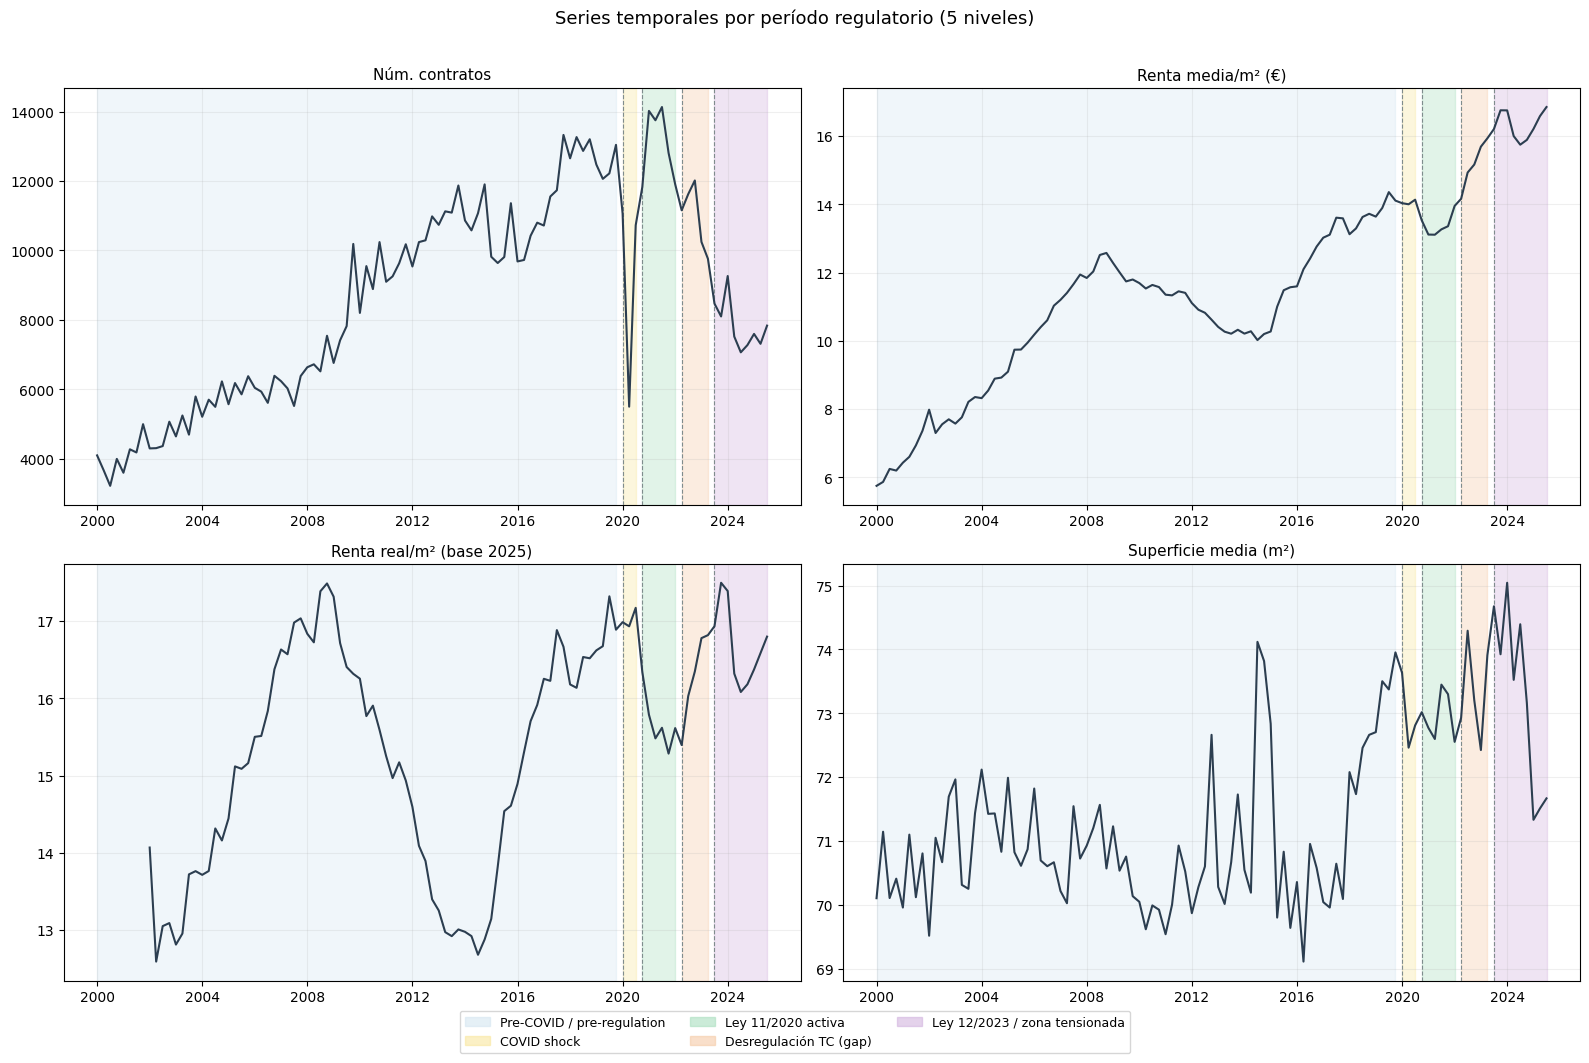
\includegraphics[width=\linewidth]{figures/fig_eda_5periods.png}
  \caption{Distribución de las variables clave por período regulatorio (boxplots).
    P3 = Ley 11/2020; P4 = Desregulación TC; P5 = Ley 12/2023.}
  \label{fig:eda_5periods}
\end{figure}

\begin{table}[H]
\caption{Tests de diferencias pre/post-regulación (ciudad)}
\label{tab:prepost}
\centering\small
\begin{threeparttable}
\begin{tabular}{lrrl}
\toprule
Variable & $\Delta$\,M (\%) & $p$-Welch & Sig. \\
\midrule
Contratos (\texttt{n})          & $+22.9$ & $0.006$ & ** \\
Precio nominal (\euro/m$^2$)    & $+41.7$ & $<.001$ & *** \\
Precio real 2025 (\euro/m$^2$)  & $+7.2$  & $<.001$ & ** \\
Superficie (m$^2$)              & $+3.0$  & $<.001$ & *** \\
\bottomrule
\end{tabular}
\begin{tablenotes}\small
\item $n_{pre}{=}83$, $n_{post}{=}20$ obs.\ trimestrales ciudad.
$^{***}p{<}.01$, $^{**}p{<}.05$.
\end{tablenotes}
\end{threeparttable}
\end{table}

El test de Chow simplificado confirma ruptura estructural en 2020Q4 para precio
nominal ($F{=}5.16$, $p{=}0.007$) y contratos ($F{=}101.2$, $p{<}0.001$), pero no
para precio real ($F{=}0.28$, $p{=}0.755$). La Figura~\ref{fig:eda_chow} muestra
los resultados del test de Chow.

\begin{figure}[H]
  \centering
  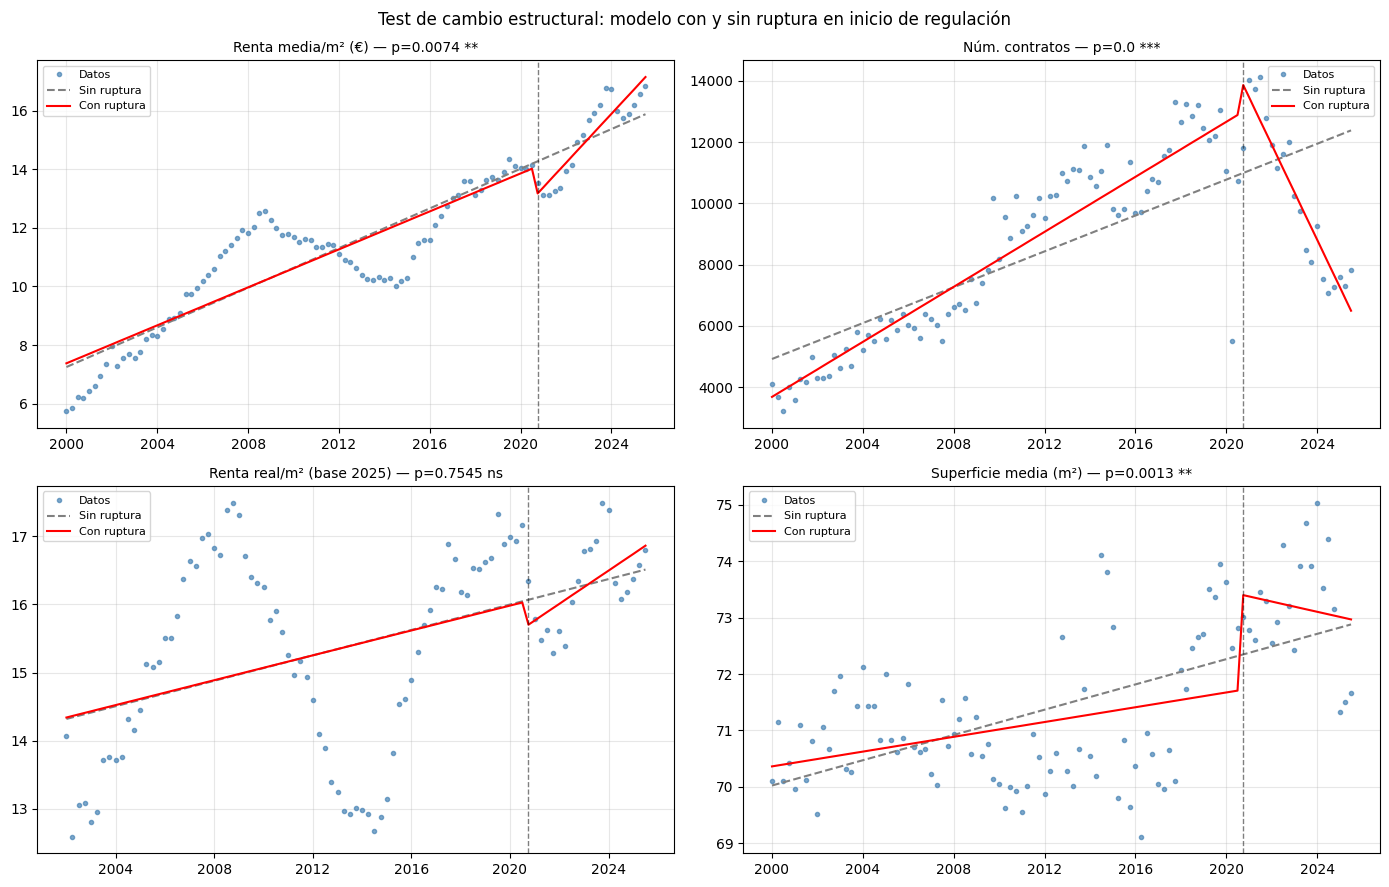
\includegraphics[width=\linewidth]{figures/fig_eda_chow.png}
  \caption{Test de Chow simplificado (ruptura 2020Q4). Las barras muestran el
    estadístico $F$ por variable; la línea roja indica el umbral $F_{0.05}$.}
  \label{fig:eda_chow}
\end{figure}

\subsection{Heterogeneidad entre distritos}

La Figura~\ref{fig:eda_districts} muestra la variación de renta real post-regulación
por distrito. Sant~Martí ($+10.8\,\%$) y Eixample ($+10.3\,\%$) lideran la variación,
mientras Nou~Barris prácticamente no varía ($+0.7\,\%$). Esta dispersión de 10~puntos
porcentuales justifica el uso del estimador \textit{within} con efectos fijos y el
análisis desagregado a nivel distrito.

\begin{figure}[H]
  \centering
  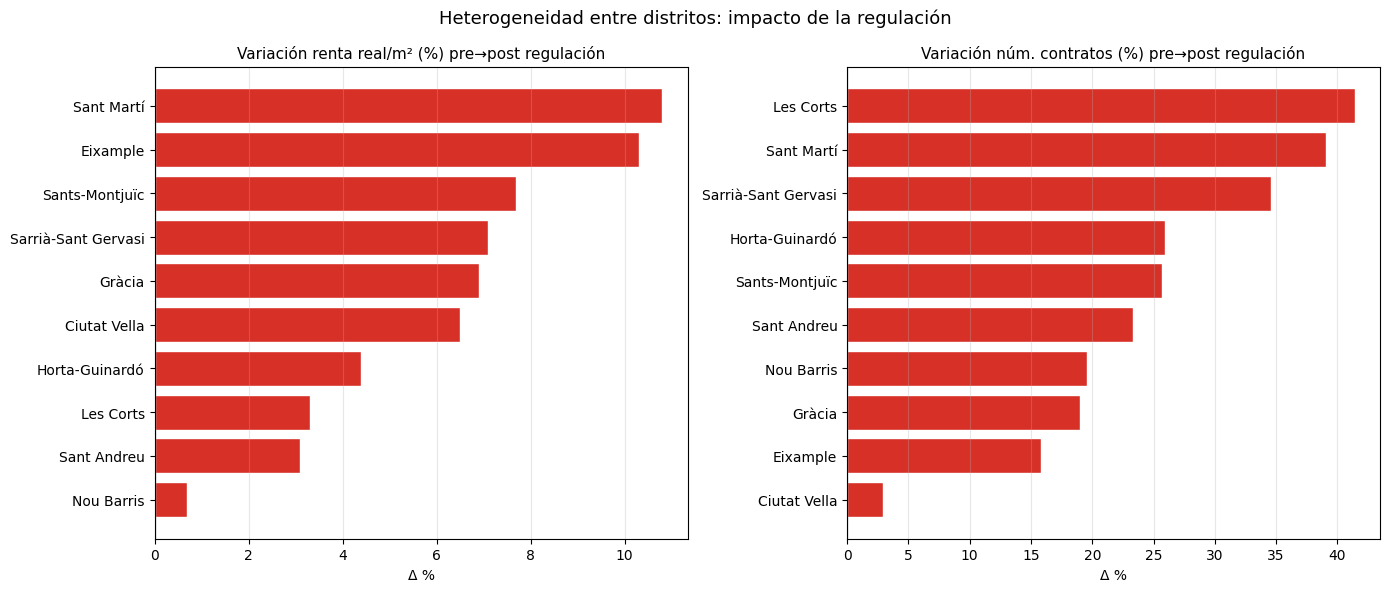
\includegraphics[width=\linewidth]{figures/fig_eda_districts.png}
  \caption{Variación (\%) de la renta real y el volumen de contratos por distrito,
    período pre vs.\ post-regulación (2020Q4--2025Q3).}
  \label{fig:eda_districts}
\end{figure}

% ===========================================================
\section{Metodología}
\label{sec:metodos}

\subsection{Módulo 1 --- Regresión de Panel con Efectos Fijos}

\subsubsection{Especificación}

Estimamos tres especificaciones sucesivas del modelo:
\begin{equation}
  y_{it} = \alpha_i + \sum_{k} \beta_k z_{k,t} + \boldsymbol{\gamma}'\mathbf{x}_{it} + \varepsilon_{it}
  \label{eq:panel_general}
\end{equation}
donde $i \in \{1,\ldots,66\}$ indexa el barrio, $t$ el trimestre, $\alpha_i$ son
efectos fijos por barrio, $z_{k,t}$ son los indicadores regulatorios y macro, y
$\mathbf{x}_{it}$ incluye controles de mercado. El estimador \textit{within}
elimina $\alpha_i$ transformando las variables en desviaciones respecto a la media
barrio-específica:
\begin{equation}
  \hat{\beta}_{WG}
  = \Bigl(\sum_i \ddot{\mathbf{X}}_i' \ddot{\mathbf{X}}_i\Bigr)^{-1}
    \sum_i \ddot{\mathbf{X}}_i' \ddot{y}_i, \qquad
  \ddot{z}_{it} = z_{it} - \bar{z}_i
  \label{eq:within}
\end{equation}
Los errores estándar se estiman con \textit{clustering} por barrio
\citep{baltagi2021econometric}, siendo robustos a heterocedasticidad y autocorrelación
intra-cluster de estructura desconocida.

La especificación más completa (M3) toma:
\begin{equation}
  y_{it} = \alpha_i + \beta_1\,\text{pr}_{t} + \beta_2\,\text{cv}_{it}
         + \beta_3\,r_{it} + \beta_4\,s_{it} + \beta_5\,e_t
         + \sum_{q=2}^{4}\!\delta_q\,Q_{qt} + \varepsilon_{it}
  \label{eq:m3}
\end{equation}
donde \texttt{pr} = \texttt{post\_regulation}, \texttt{cv} = \texttt{covid\_dummy},
$r$ = precio por m$^2$, $s$ = superficie, $e$ = Euríbor y $Q_q$ son dummies
estacionales trimestrales.

\subsubsection{Modelo M4 --- tres regímenes}

Para descomponer el efecto temporal, reemplazamos \texttt{post\_regulation} por tres
indicadores de régimen:
\begin{equation}
  y_{it} = \alpha_i + \delta_1 D_{11,t} + \delta_2 D_{tc,t} + \delta_3 D_{12,t}
         + \boldsymbol{\gamma}'\mathbf{x}_{it} + \varepsilon_{it}
  \label{eq:m4}
\end{equation}
donde $D_{11}$, $D_{tc}$ y $D_{12}$ son indicadores de los períodos P3, P4 y P5
respectivamente (Tabla~\ref{tab:periodos_app}).

\subsection{Módulo 2 --- Clasificación de Tensión Contractual}

\subsubsection{Variable objetivo}

Definimos un episodio de tensión contractual para el barrio $i$ en el trimestre $t$:
\begin{equation}
  \tau_{it} = \mathbf{1}\!\left[
    \frac{n_{it} - n_{i,t-4}}{n_{i,t-4}} < \hat{q}_{25,i}^{(\leq 2019)}
    \;\wedge\;
    \frac{n_{it} - n_{i,t-4}}{n_{i,t-4}} < -0.05
  \right]
  \label{eq:tension}
\end{equation}
El umbral $\hat{q}_{25,i}^{(\leq 2019)}$ es el percentil 25 de la distribución
histórica del barrio $i$ calculado sobre el período pre-regulación; el corte del
$-5\,\%$ evita activaciones por fluctuaciones menores.

\subsubsection{Algoritmos y evaluación}

Entrenamos tres clasificadores con split temporal estricto ($\text{train}\leq 2021$,
$\text{test}\geq 2022$): Regresión Logística L2 (RL), Random Forest (RF,
200~árboles, profundidad máxima 6, \texttt{class\_weight='balanced'}) y Gradient
Boosting (GB). La métrica principal es el ROC-AUC:
\begin{equation}
  \text{AUC} = \int_0^1 \text{TPR}(t)\, d\,\text{FPR}(t)
  \label{eq:auc}
\end{equation}
La validación de estabilidad temporal usa \texttt{TimeSeriesSplit} con $K{=}5$
folds \citep{bergmeir2018note}. La importancia de variables se estima por
permutación sobre el test para evitar el sesgo del criterio de impureza del árbol.

\subsection{Módulo 3 --- SARIMAX e ITS-3 a nivel Distrito}

\subsubsection{Tests de estacionariedad}

Antes de especificar el modelo, verificamos el orden de integración de cada serie
con el protocolo doble ADF+KPSS:
\begin{align}
  \text{ADF:}&\quad H_0: \gamma = 0 \text{ (raíz unitaria)} \nonumber\\
  &\quad \Delta y_t = \mu + \gamma y_{t-1} + \sum_{j=1}^p \phi_j \Delta y_{t-j} + \varepsilon_t
  \label{eq:adf}\\
  \text{KPSS:}&\quad H_0: \text{serie estacionaria en torno a tendencia}
  \label{eq:kpss}
\end{align}
La regla de decisión es: I(1) si ADF no rechaza en niveles \textit{y} KPSS rechaza
en niveles \textit{y} ADF rechaza en primera diferencia.

\subsubsection{Especificación SARIMAX}

Para cada par $(d, m)$ con $d \in \mathcal{D}$ (10 distritos) y $m \in \mathcal{M}$
(3 métricas), estimamos:
\begin{equation}
  \phi(B)\,\Phi(B^4)\,(1{-}B)\,y_{d,t}
  = c_d + \theta(B)\,\Theta(B^4)\,\varepsilon_{d,t}
    + \gamma_d\,e_t
  \label{eq:sarimax}
\end{equation}
donde los operadores de retardo son:
\begin{align*}
  \phi(B)   &= 1 - \phi_1 B        & \text{(AR no estacional, }p{=}1\text{)}\\
  \Phi(B^4) &= 1 - \Phi_1 B^4      & \text{(AR estacional, }P{=}1\text{)}\\
  \theta(B) &= 1 + \theta_1 B      & \text{(MA no estacional, }q{=}1\text{)}\\
  \Theta(B^4)&= 1 + \Theta_1 B^4  & \text{(MA estacional, }Q{=}1\text{)}\\
  (1{-}B)   &                      & \text{(diferencia regular, }d{=}1\text{)}
\end{align*}
y $e_t$ es el Euríbor~12m. El orden $(d{=}1)$ queda justificado por los tests
ADF+KPSS en 29 de 30 combinaciones (Tabla~\ref{tab:stat_orden_app}). La estimación
usa MLE con matrix de covarianza OIM (\texttt{cov\_type='oim'}), más estable que el
estimador OPG en muestras moderadas \citep{harvey1989forecasting}.

Los cortes son: $\text{train} < \text{2020Q1}$, test SARIMAX $\geq \text{2020Q1}$
y test baselines $\geq \text{2022Q1}$ (para excluir el shock COVID de la evaluación
de naïve y ETS). Las métricas de evaluación son:
\begin{align}
  \MAPE &= \frac{100}{T}\sum_{t=1}^T \left|\frac{y_t - \hat{y}_t}{y_t}\right|
  \label{eq:mape}\\
  \RMSE &= \sqrt{\frac{1}{T}\sum_{t=1}^T (y_t - \hat{y}_t)^2}
  \label{eq:rmse}
\end{align}

\subsubsection{ITS-3 multi-ruptura}

El modelo de series temporales interrumpidas con tres rupturas especifica:
\begin{equation}
  y_t^{(m)} = \beta_0 + \beta_1 t
    + \sum_{k \in \mathcal{K}}\!\bigl[\beta_{2k} D_{k,t} + \beta_{3k}\,t_{k,t}^+\bigr]
    + \beta_4\,\text{cv}_t + \beta_5\,e_t + \varepsilon_t
  \label{eq:its3}
\end{equation}
con $\mathcal{K}{=}\{ley11, tc, ley12\}$, $D_{k,t}{=}\mathbf{1}[t{\geq}t_k^*]$
(función escalón) y $t_{k,t}^+{=}\max(0,t{-}t_k^*)$ (rampa post-ruptura). Los
coeficientes $\beta_{2k}$ miden el cambio inmediato de nivel (\textit{level shift})
y $\beta_{3k}$ el cambio de pendiente tras la ruptura $k$.

Los errores se estiman con la corrección HAC de Newey-West con $L{=}4$ lags:
\begin{equation}
  \hat{V}_{HAC} = (X'X)^{-1} \hat{\Omega}_{NW} (X'X)^{-1}, \quad
  \hat{\Omega}_{NW} = \sum_{l=-L}^{L} w_l \hat{\Gamma}_l
  \label{eq:hac}
\end{equation}
con pesos de Bartlett $w_l = 1 - |l|/(L{+}1)$ y $\hat{\Gamma}_l$ la estimación
de la autocovarianza de lag $l$ de los residuos OLS \citep{newey1987hac}.

\subsection{Módulo 4 --- Series Temporales Ciudad Agregada}

Replicamos los modelos del Módulo~3 sobre la serie ciudad construida como:
\begin{equation}
  \bar{y}_t^{(m)} = \frac{\sum_{d} n_{d,t}\, y_{d,t}^{(m)}}{\sum_{d} n_{d,t}}
  \label{eq:city_weighted}
\end{equation}
proporcionando una capa de validación cruzada: si los coeficientes ITS-3 ciudad son
coherentes con la mediana de los coeficientes distrito, la narrativa global es
robusta; si divergen, existe heterogeneidad geográfica relevante que el agregado
enmascara.

% ===========================================================
\section{Resultados Experimentales}
\label{sec:resultados}

\subsection{Módulo 1: Panel de Datos}

La Tabla~\ref{tab:panel} presenta las estimaciones para M1, M2 y M3.

\begin{table}[H]
\caption{Modelos de panel FE (var.\ dep.: $\Delta^4\!\log n_{it}$)}
\label{tab:panel}
\centering\small
\begin{threeparttable}
\begin{tabular}{lccc}
\toprule
 & M1 & M2 & M3 \\
\midrule
\texttt{post\_reg.}  & $-0.015$ & $0.136^{***}$ & $0.231^{***}$ \\
                     & $(-1.89)$ & $(9.96)$ & $(15.71)$ \\
\texttt{covid}       & $0.204^{***}$ & $0.159^{***}$ & $0.040^{**}$ \\
                     & $(13.4)$ & $(10.0)$ & $(2.29)$ \\
$r_{it}$            & --- & $-0.066^{***}$ & $-0.038^{***}$ \\
$s_{it}$            & --- & $-0.005$ & $-0.003$ \\
$e_t$               & --- & --- & $-0.076^{***}$ \\
                     & & & $(-7.96)$ \\
Efectos estacionales & No & No & Sí \\
\midrule
$R^2$ Within & $.029$ & $.089$ & $.128$ \\
Obs.         & 2,838 & 2,838 & 2,838 \\
\bottomrule
\end{tabular}
\begin{tablenotes}\small
\item $t$-estadísticos entre paréntesis, SE \textit{clustered} por barrio.
$^{***}p{<}.01$, $^{**}p{<}.05$.
Efectos fijos por barrio en todos los modelos (estimador \textit{within}).
\end{tablenotes}
\end{threeparttable}
\end{table}

El cambio de signo de \texttt{post\_regulation} entre M1 ($-0.015$, ns) y M3
($+0.231$, $p{<}.001$) responde a la mediación del precio: una vez que controlamos
por $r_{it}$, emerge el efecto directo de la regulación sobre la rotación del
segmento que permanece en el mercado observable. La elasticidad precio-contratos
es $\hat{\beta}_3 {=} -0.038$ ($p{<}.001$), coherente con la predicción de la teoría:
precios más elevados reducen el ritmo de nuevas contrataciones.

El Euríbor tiene un efecto directo negativo sobre los contratos ($\hat{\beta}_5{=}-0.076$,
$p{<}.001$): un aumento de 100 puntos básicos en el Euríbor a 12m se asocia, \textit{ceteris
paribus}, con una caída de $7.6$ puntos porcentuales en el crecimiento de contratos. Esto
es el canal financiero: cuando el coste de la hipoteca sube, más hogares presionan el
mercado de alquiler pero simultáneamente más propietarios posponen la puesta en alquiler
de segunda vivienda.

La Figura~\ref{fig:panel_resid} muestra el análisis de residuos del modelo M3.

\begin{figure}[H]
  \centering
  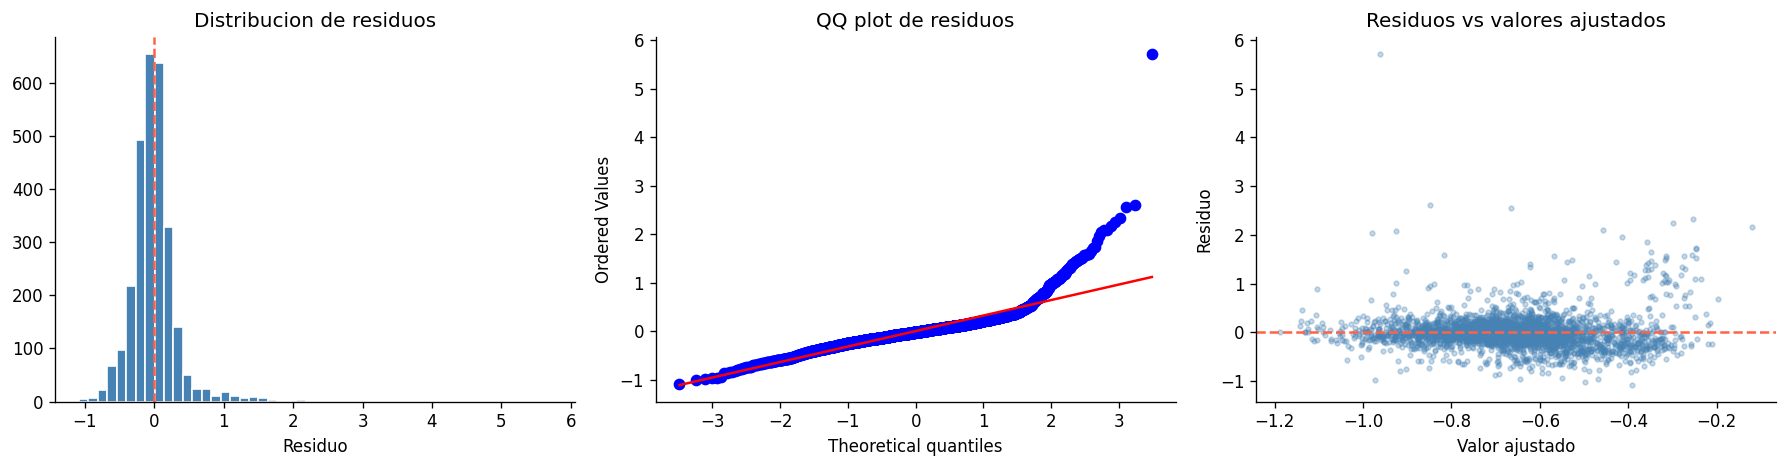
\includegraphics[width=\linewidth]{figures/fig02_residuos_panel.png}
  \caption{Diagnóstico de residuos del modelo M3. Arriba: residuos vs.\ ajustados;
    abajo: distribución de residuos estandarizados. La línea roja es la mediana
    y la banda gris el intervalo $[\pm 1.5\,\sigma]$.}
  \label{fig:panel_resid}
\end{figure}

\textbf{Modelo M4.} La descomposición por regímenes produce $\hat{\delta}_1{=}+0.317$
(Ley~11/2020, $p{<}.001$), $\hat{\delta}_2{=}+0.001$ (derogación~TC, ns) y
$\hat{\delta}_3{=}+0.028$ (Ley~12/2023, ns). La significancia exclusiva del régimen
P3 en el estimador \textit{within} refleja que el rebote post-COVID de 2020Q4 coincide
con la entrada en vigor de la Ley~11/2020, haciendo difícil separar ambos efectos.

\subsection{Módulo 2: Clasificación}

\begin{table}[H]
\caption{Métricas de clasificación (test $\geq$2022Q1, $n{=}990$)}
\label{tab:clf}
\centering\small
\begin{threeparttable}
\begin{tabular}{lccc}
\toprule
Modelo & AUC & AP & F1 \\
\midrule
Log.\ L2     & \textbf{0.606} & 0.750 & 0.765 \\
Random Forest& 0.553 & 0.663 & 0.748 \\
Grad.\ Boost.& 0.573 & 0.680 & 0.752 \\
\bottomrule
\end{tabular}
\begin{tablenotes}\small
\item AUC-CV temporal (5 folds, RF): $0.564 \pm 0.060$.
AP = Average Precision.
\end{tablenotes}
\end{threeparttable}
\end{table}

Los tres clasificadores convergen en un AUC moderado (0.55--0.61), coherente con la
dificultad intrínseca del problema: la tensión contractual en mercados regulados tiene
un componente genuinamente impredecible vinculado a decisiones individuales de los
propietarios. La Figura~\ref{fig:roc} muestra las curvas ROC completas.

\begin{figure}[H]
  \centering
  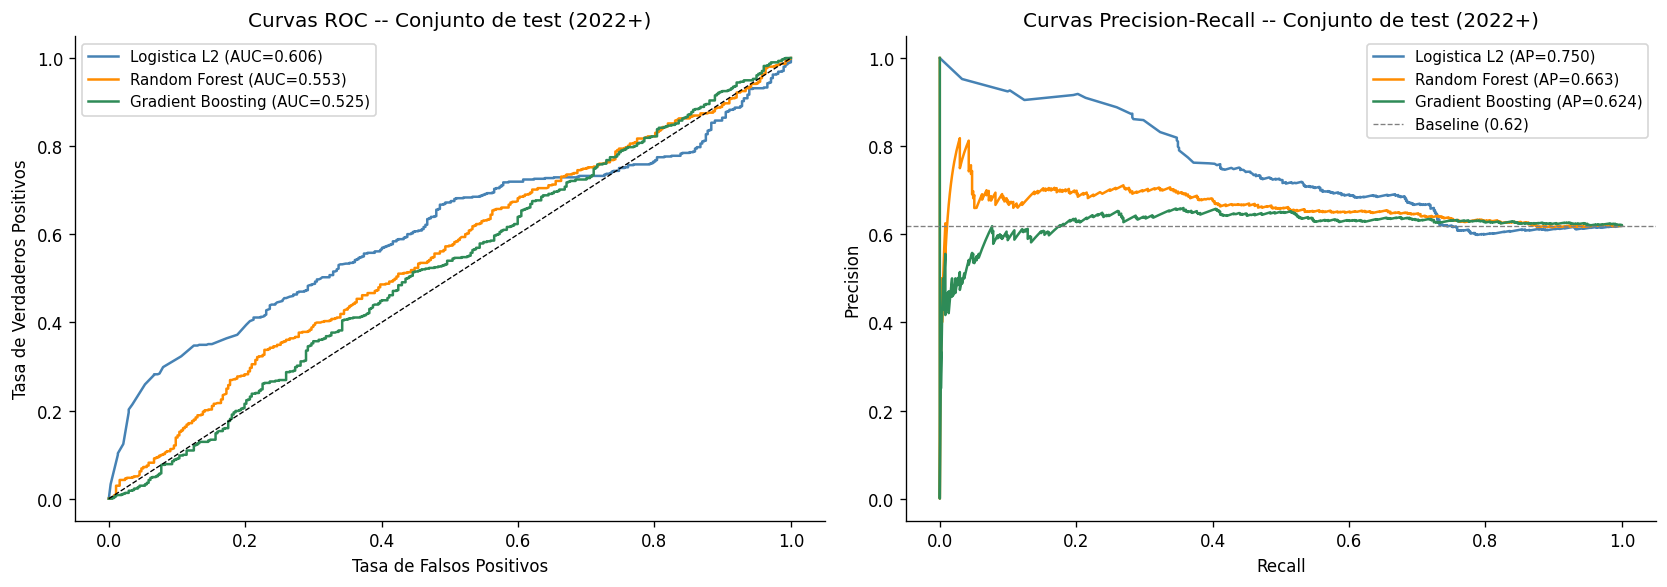
\includegraphics[width=\linewidth]{figures/fig03_roc_curves.png}
  \caption{Curvas ROC (izquierda) y Precision-Recall (derecha) para los tres
    clasificadores sobre el test 2022--2025. La línea punteada diagonal es el
    clasificador aleatorio (AUC = 0.50).}
  \label{fig:roc}
\end{figure}

La Figura~\ref{fig:perm} muestra la importancia por permutación. El precio real
domina claramente ($\text{imp}{=}0.063\pm 0.012$), seguido de Euríbor ($0.004$) y
$D_{ley11}$ ($0.003$). El hecho de que $D_{ley12}$ y $D_{tc}$ tengan importancia
nula no indica que no tengan efecto: simplemente que, dado el precio real, no aportan
información adicional al clasificador --- la mediación es completa a través del precio.

\begin{figure}[H]
  \centering
  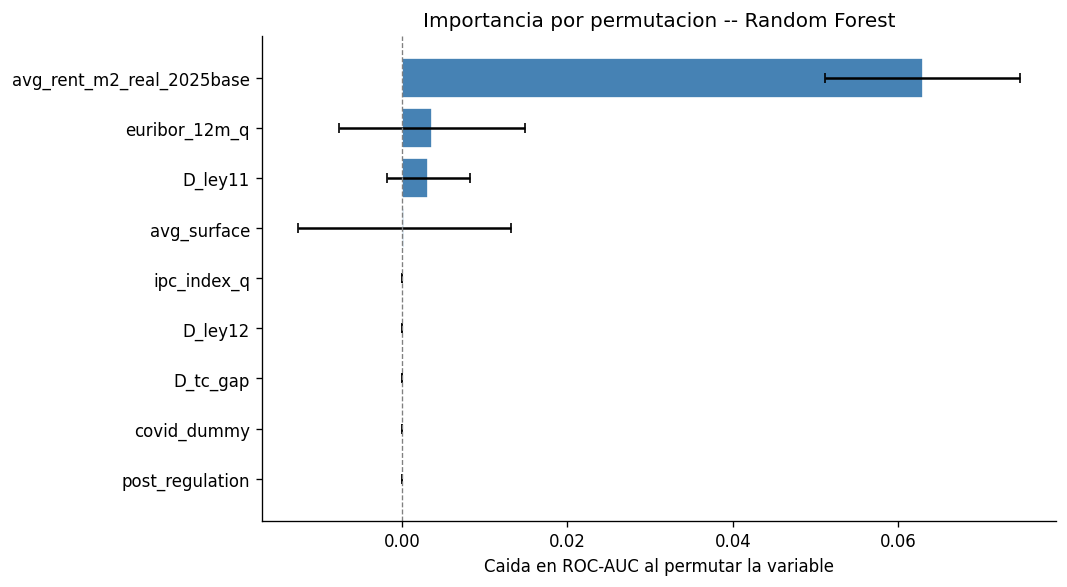
\includegraphics[width=0.9\linewidth]{figures/fig04_permutation.png}
  \caption{Importancia por permutación (Random Forest, test 2022--2025, 20
    repeticiones). El precio real base~2025 es la variable dominante.}
  \label{fig:perm}
\end{figure}

\subsection{Módulo 3: Series Temporales Distrito}

\subsubsection{Estacionariedad y ACF/PACF}

Los tests ADF+KPSS confirman I(1) en 10/10 distritos para precio nominal y contratos,
y en 8/10 para precio real (1 I(0) y 1 ambiguo). La Figura~\ref{fig:acf} muestra el
ACF y PACF en primera diferencia para Eixample. El pico significativo en lag~4 confirma
la estacionalidad anual que motiva el término $(P,D,Q)_4$ del SARIMAX.

\begin{figure}[H]
  \centering
  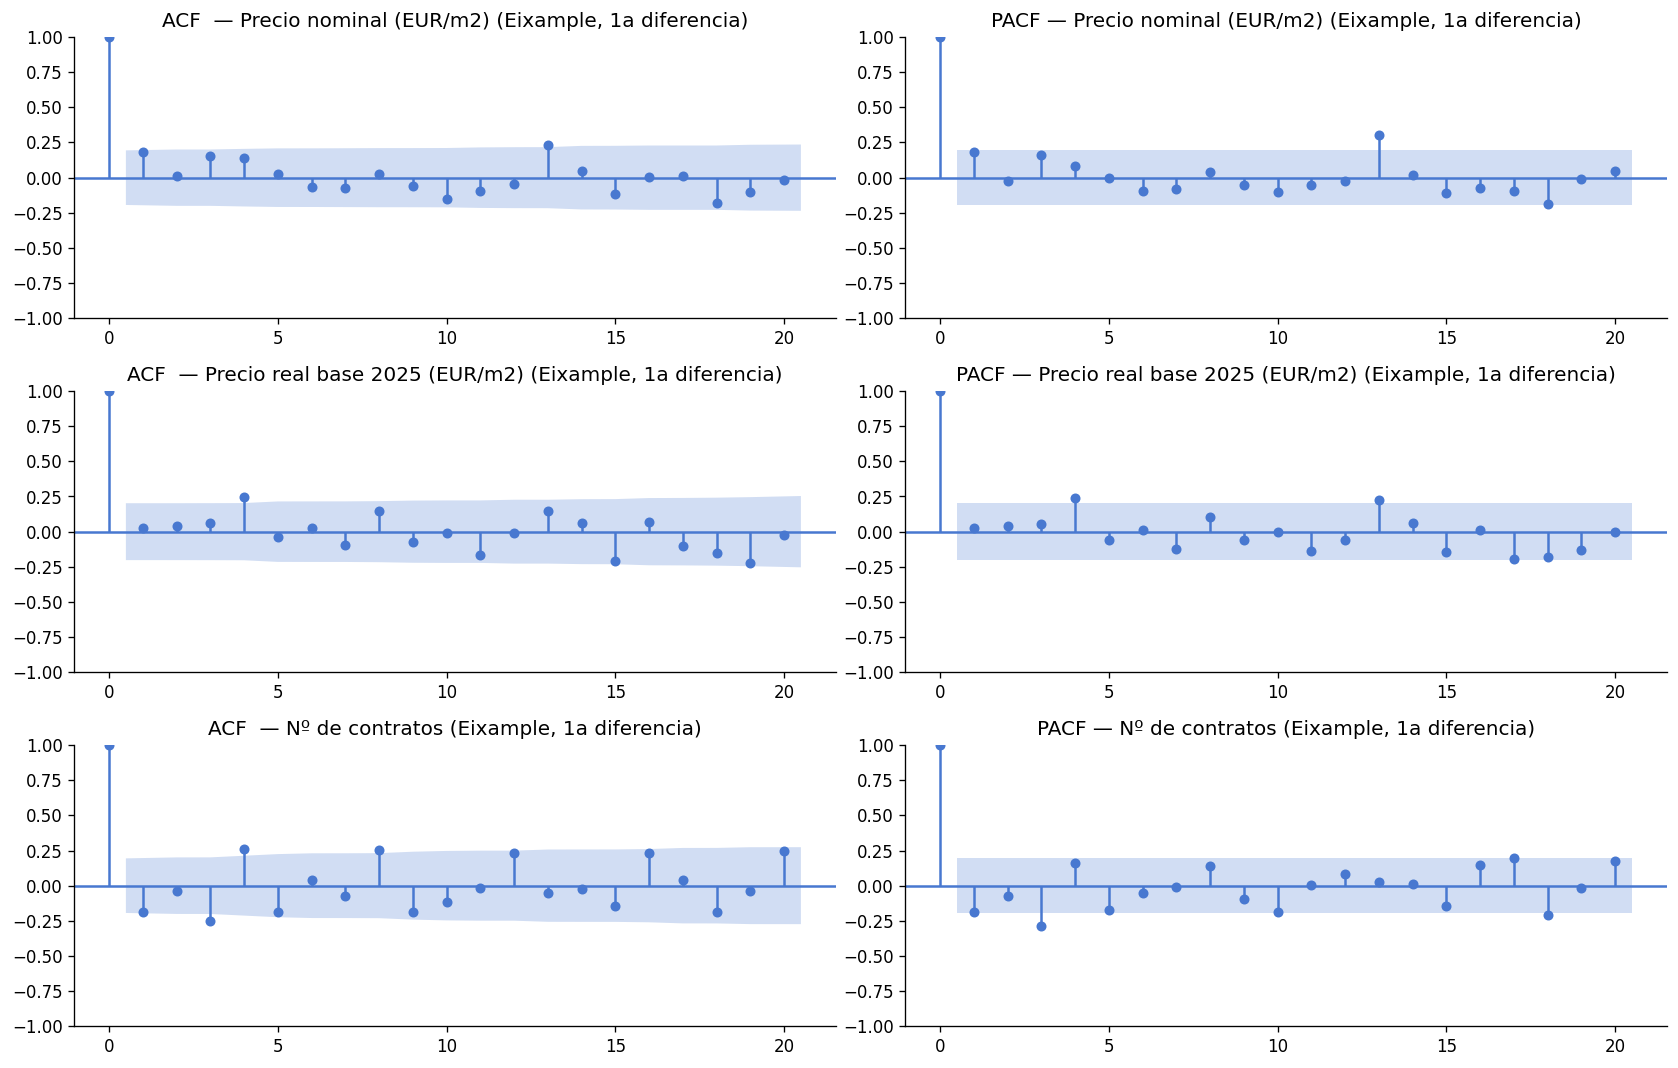
\includegraphics[width=\linewidth]{figures/fig05_acf_pacf.png}
  \caption{ACF y PACF en primera diferencia para Eixample (3 métricas, fila por
    métrica). El lag~4 significativo en todas las métricas justifica el orden
    estacional $(1,0,1)_4$.}
  \label{fig:acf}
\end{figure}

\subsubsection{Comparativa de modelos por distrito}

La Tabla~\ref{tab:mape_dist} resume el MAPE por distrito para el precio nominal.

\begin{table}[H]
\caption{MAPE (\%) precio nominal por distrito (test 2022Q1+)}
\label{tab:mape_dist}
\centering\small
\begin{tabular}{lrrr}
\toprule
Distrito & Naïve & ETS & SARIMAX \\
\midrule
Gràcia          & 7.45 & 8.29 & \textbf{2.82} \\
Eixample        & 7.16 & 4.21 & \textbf{3.49} \\
Ciutat Vella    & 8.37 & 6.19 & \textbf{3.96} \\
Sant Martí      & 7.40 & -- & \textbf{2.90} \\
Sants-Montjuïc  & 8.40 & 9.82 & \textbf{4.10} \\
Les Corts       & 7.12 & 5.23 & 9.02 \\
Horta-Guinardó  & 6.44 & \textbf{4.40} & 9.38 \\
Nou Barris      & 6.56 & \textbf{3.49} & 8.70 \\
Sant Andreu     & 6.22 & \textbf{3.48} & 8.60 \\
Sarrià-S.G.     & -- & -- & \textbf{7.40} \\
\bottomrule
\end{tabular}
\end{table}

El SARIMAX gana en 6/10 distritos para precio nominal, el ETS en 4/10 (periféricos).
Para precio real, el naïve gana en 7/10; para contratos, el naïve domina en 10/10.
Este patrón es teóricamente coherente: el Euríbor aporta información sobre el nivel
monetario del precio pero no sobre el volumen de contratos, que depende de decisiones
de oferta más difíciles de modelar con variables macro.

\subsection{Módulo 4: Series Temporales Ciudad}

\subsubsection{Diagnóstico SARIMAX}

La Figura~\ref{fig:diag} muestra los paneles de diagnóstico de residuos del SARIMAX
para las tres métricas. Los estadísticos Ljung-Box: $p(\text{lag8}){=}0.985$ (nominal),
$p{=}0.995$ (real), $p{=}0.994$ (contratos) confirman la ausencia de autocorrelación
residual a nivel ciudad.

\begin{figure}[H]
  \centering
  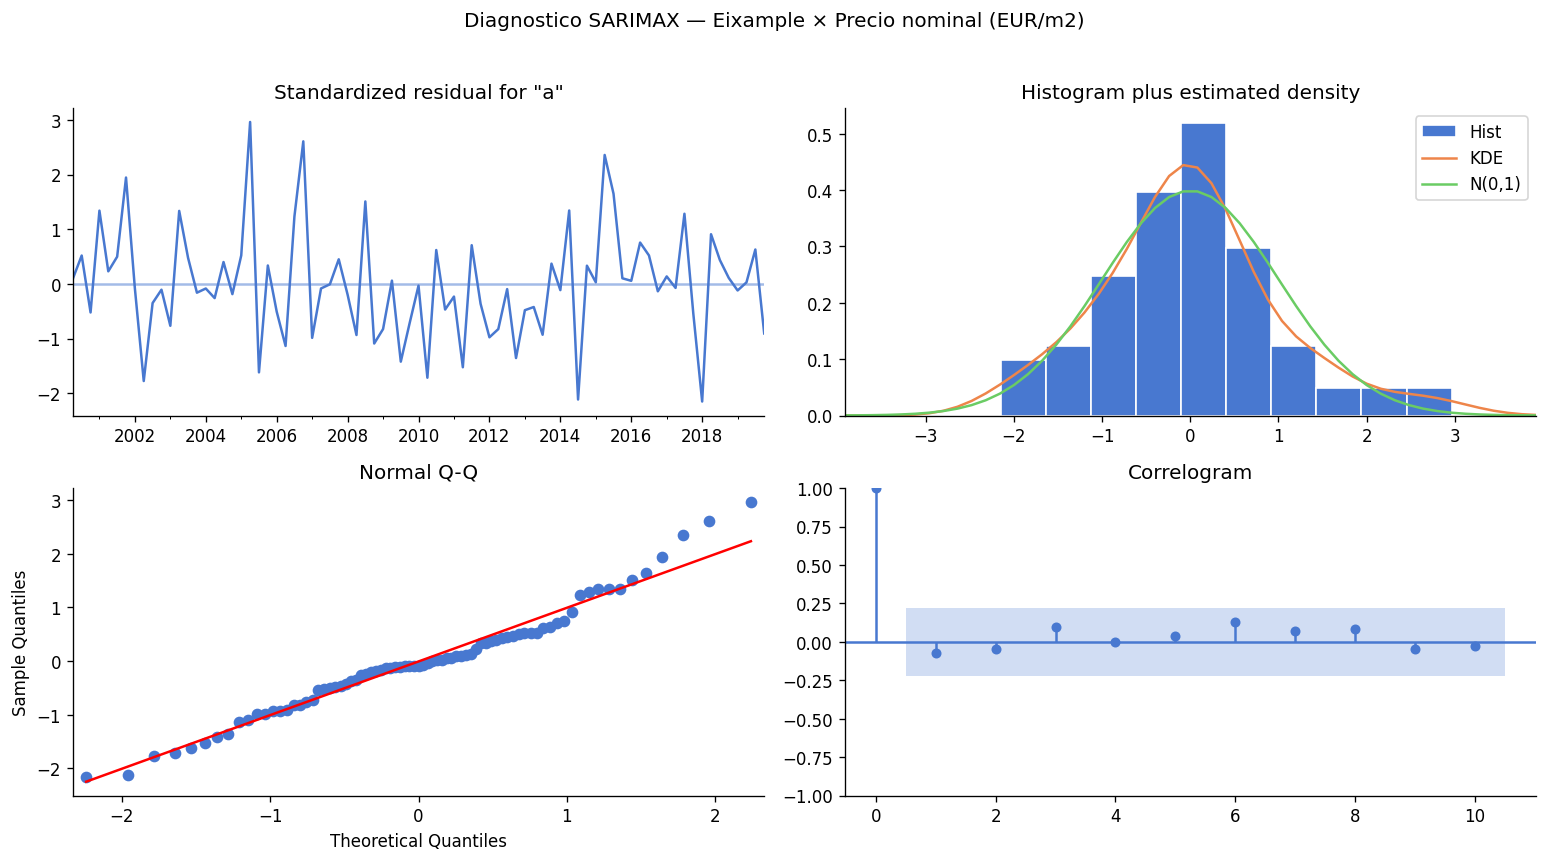
\includegraphics[width=\linewidth]{figures/fig09_diagnostics_sarimax.png}
  \caption{Diagnóstico SARIMAX para Eixample $\times$ precio nominal (representativo).
    De izquierda a derecha y de arriba a abajo: residuos estandarizados, histograma
    $+$ KDE, Q-Q plot y correlograma. Los residuos se comportan como ruido blanco.}
  \label{fig:diag}
\end{figure}

\subsubsection{Comparativa de modelos ciudad}

\begin{table}[H]
\caption{Comparativa de modelos ciudad (test 2022Q1--2025Q3)}
\label{tab:ciudad_comp}
\centering\small
\begin{threeparttable}
\begin{tabular}{lrrrl}
\toprule
Métrica & Naïve & ETS & SARIMAX & Best \\
\midrule
Nominal (\euro/m$^2$) & 6.97 & 6.08 & \textbf{3.29} & SAR \\
Real 2025 (\euro/m$^2$)& 4.67 & \textbf{4.45} & 6.01 & ETS \\
Contratos              & \textbf{19.43} & 51.53 & 56.83 & Naïve \\
\bottomrule
\end{tabular}
\begin{tablenotes}\small
\item MAPE (\%). SARIMAX nominal: AIC$=12.1$, BIC$=28.7$.
\end{tablenotes}
\end{threeparttable}
\end{table}

La Figura~\ref{fig:sarimax_city} compara las predicciones SARIMAX y ETS con la
serie real ciudad bajo las bandas de períodos regulatorios.

\begin{figure}[H]
  \centering
  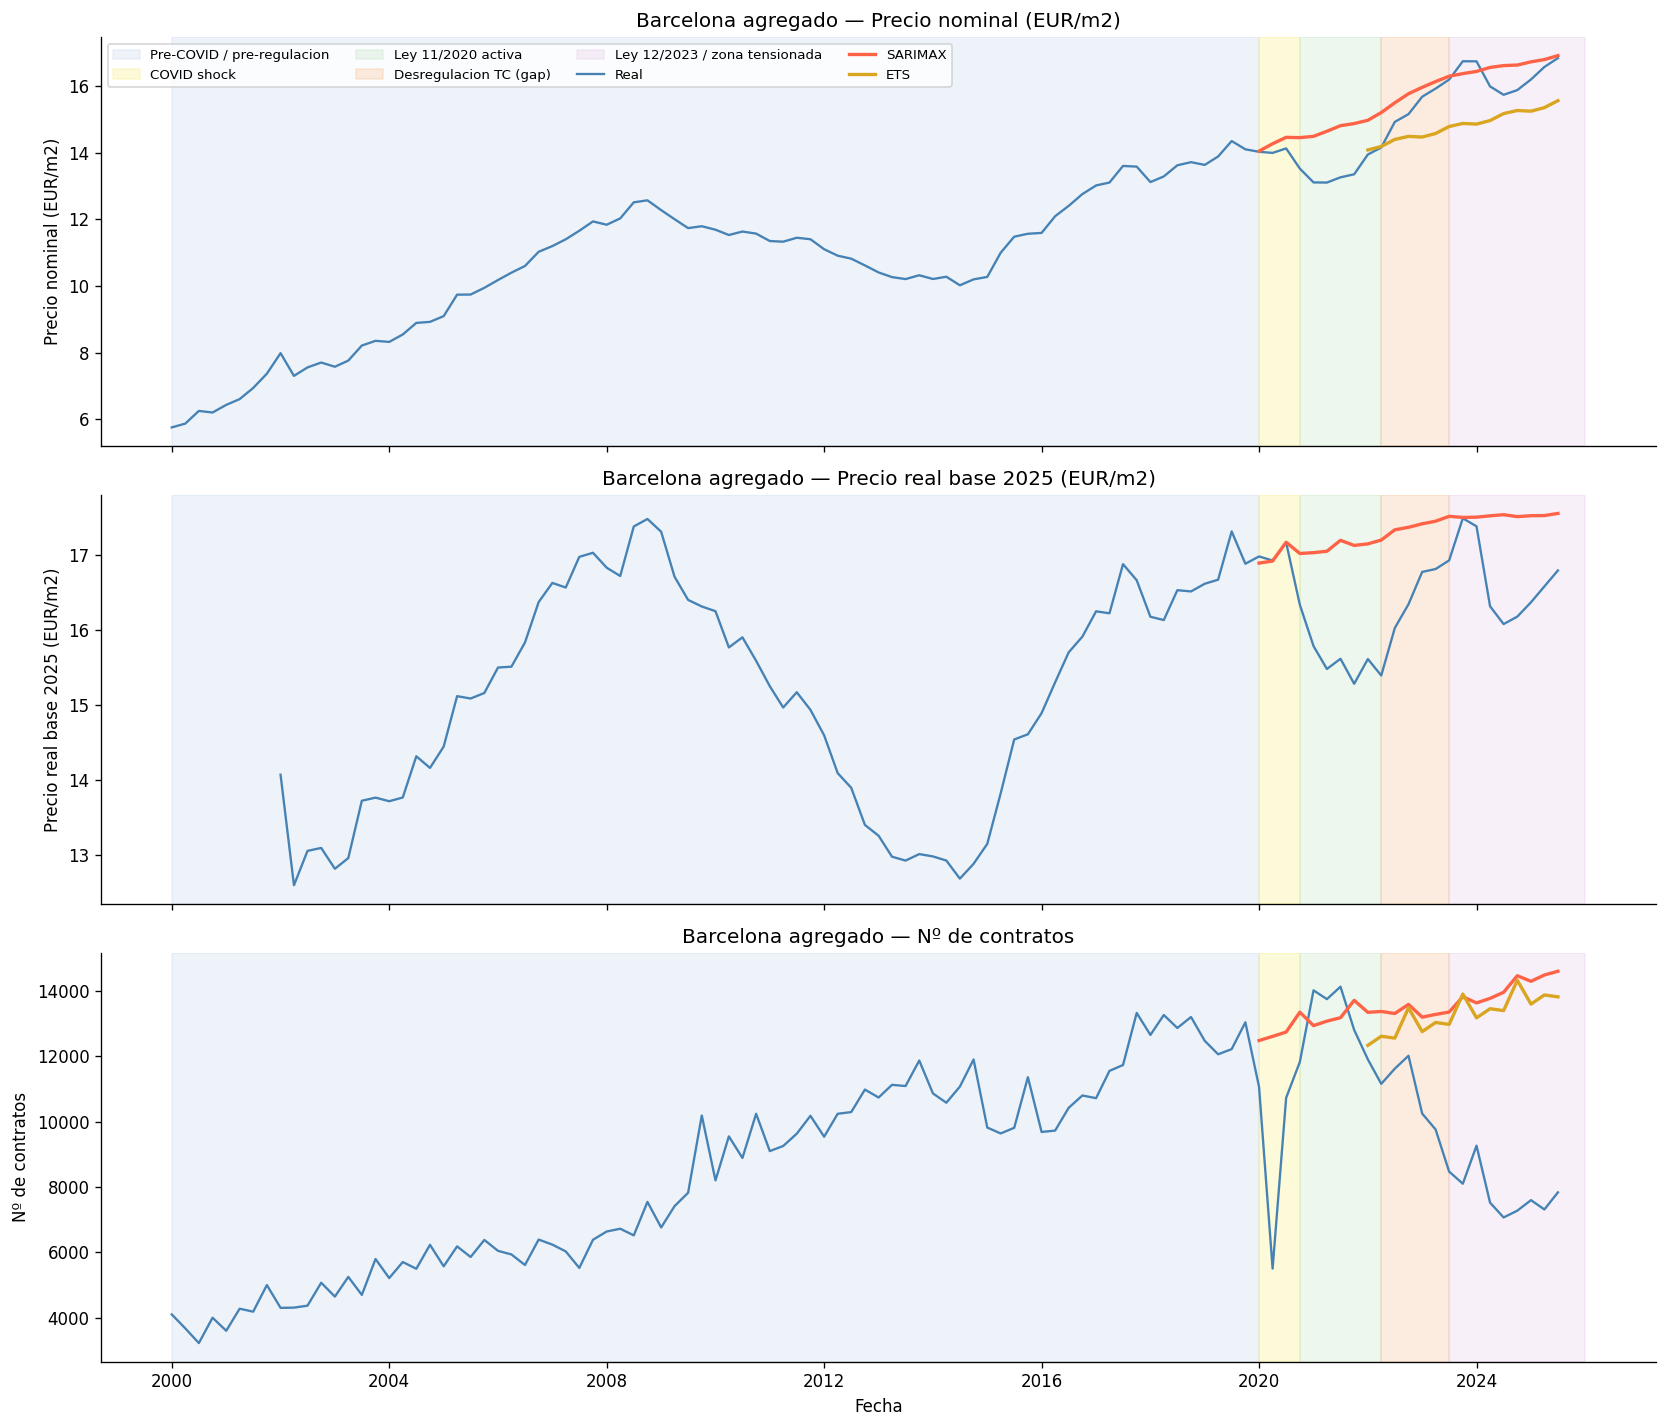
\includegraphics[width=\linewidth]{figures/fig06_sarimax_city.png}
  \caption{Predicciones out-of-sample ciudad (3 métricas). La línea azul es la
    serie observada; rojo = SARIMAX; amarillo = ETS. Las bandas de color señalan
    los cinco períodos regulatorios.}
  \label{fig:sarimax_city}
\end{figure}

\subsubsection{ITS-3: análisis de intervención}

La Tabla~\ref{tab:its3} reporta los coeficientes de las tres rupturas regulatorias
para las tres métricas. La Figura~\ref{fig:its3_city} visualiza el ajustado frente
al contrafactual (trayectoria pre-intervención proyectada hacia adelante).

\begin{table}[H]
\caption{ITS-3 ciudad: level shifts y rampas (HAC NW, $L{=}4$)}
\label{tab:its3}
\centering\small
\begin{threeparttable}
\begin{tabular}{lrclrcl}
\toprule
 & \multicolumn{3}{c}{Nominal} & \multicolumn{3}{c}{Real 2025} \\
\cmidrule(lr){2-4}\cmidrule(lr){5-7}
 & $\hat\beta$ & $p$ & & $\hat\beta$ & $p$ & \\
\midrule
$D_{ley11}$     & $-1.112$ & $.007$ & ** & $-0.041$ & $.942$ & \\
$t^+_{ley11}$   & $-0.049$ & $.381$ &    & $-0.235$ & $.000$ & ***\\
$D_{tc}$        & $-0.037$ & $.881$ &    & $-0.558$ & $.003$ & **\\
$t^+_{tc}$      & $-0.232$ & $.134$ &    & $-0.299$ & $.021$ & **\\
$D_{ley12}$     & $+0.383$ & $.102$ & $^\dag$ & $+0.495$ & $.034$ & *\\
$t^+_{ley12}$   & $+0.360$ & $.068$ & $^\dag$ & $+0.630$ & $.000$ & ***\\
\texttt{eurib.} & $+0.654$ & $.000$ & *** & $+0.911$ & $.000$ & ***\\
\midrule
$R^2$           & \multicolumn{3}{c}{0.904} & \multicolumn{3}{c}{0.513} \\
\bottomrule
\end{tabular}
\begin{tablenotes}\small
\item $^{***}p{<}.01$, $^{**}p{<}.05$, $^{*}p{<}.10$, $^\dag p{<}.15$.
Para contratos: $D_{ley12}{=}{-}1.588$ ($p{=}.007$, **), $R^2{=}0.918$.
\end{tablenotes}
\end{threeparttable}
\end{table}

\begin{figure}[H]
  \centering
  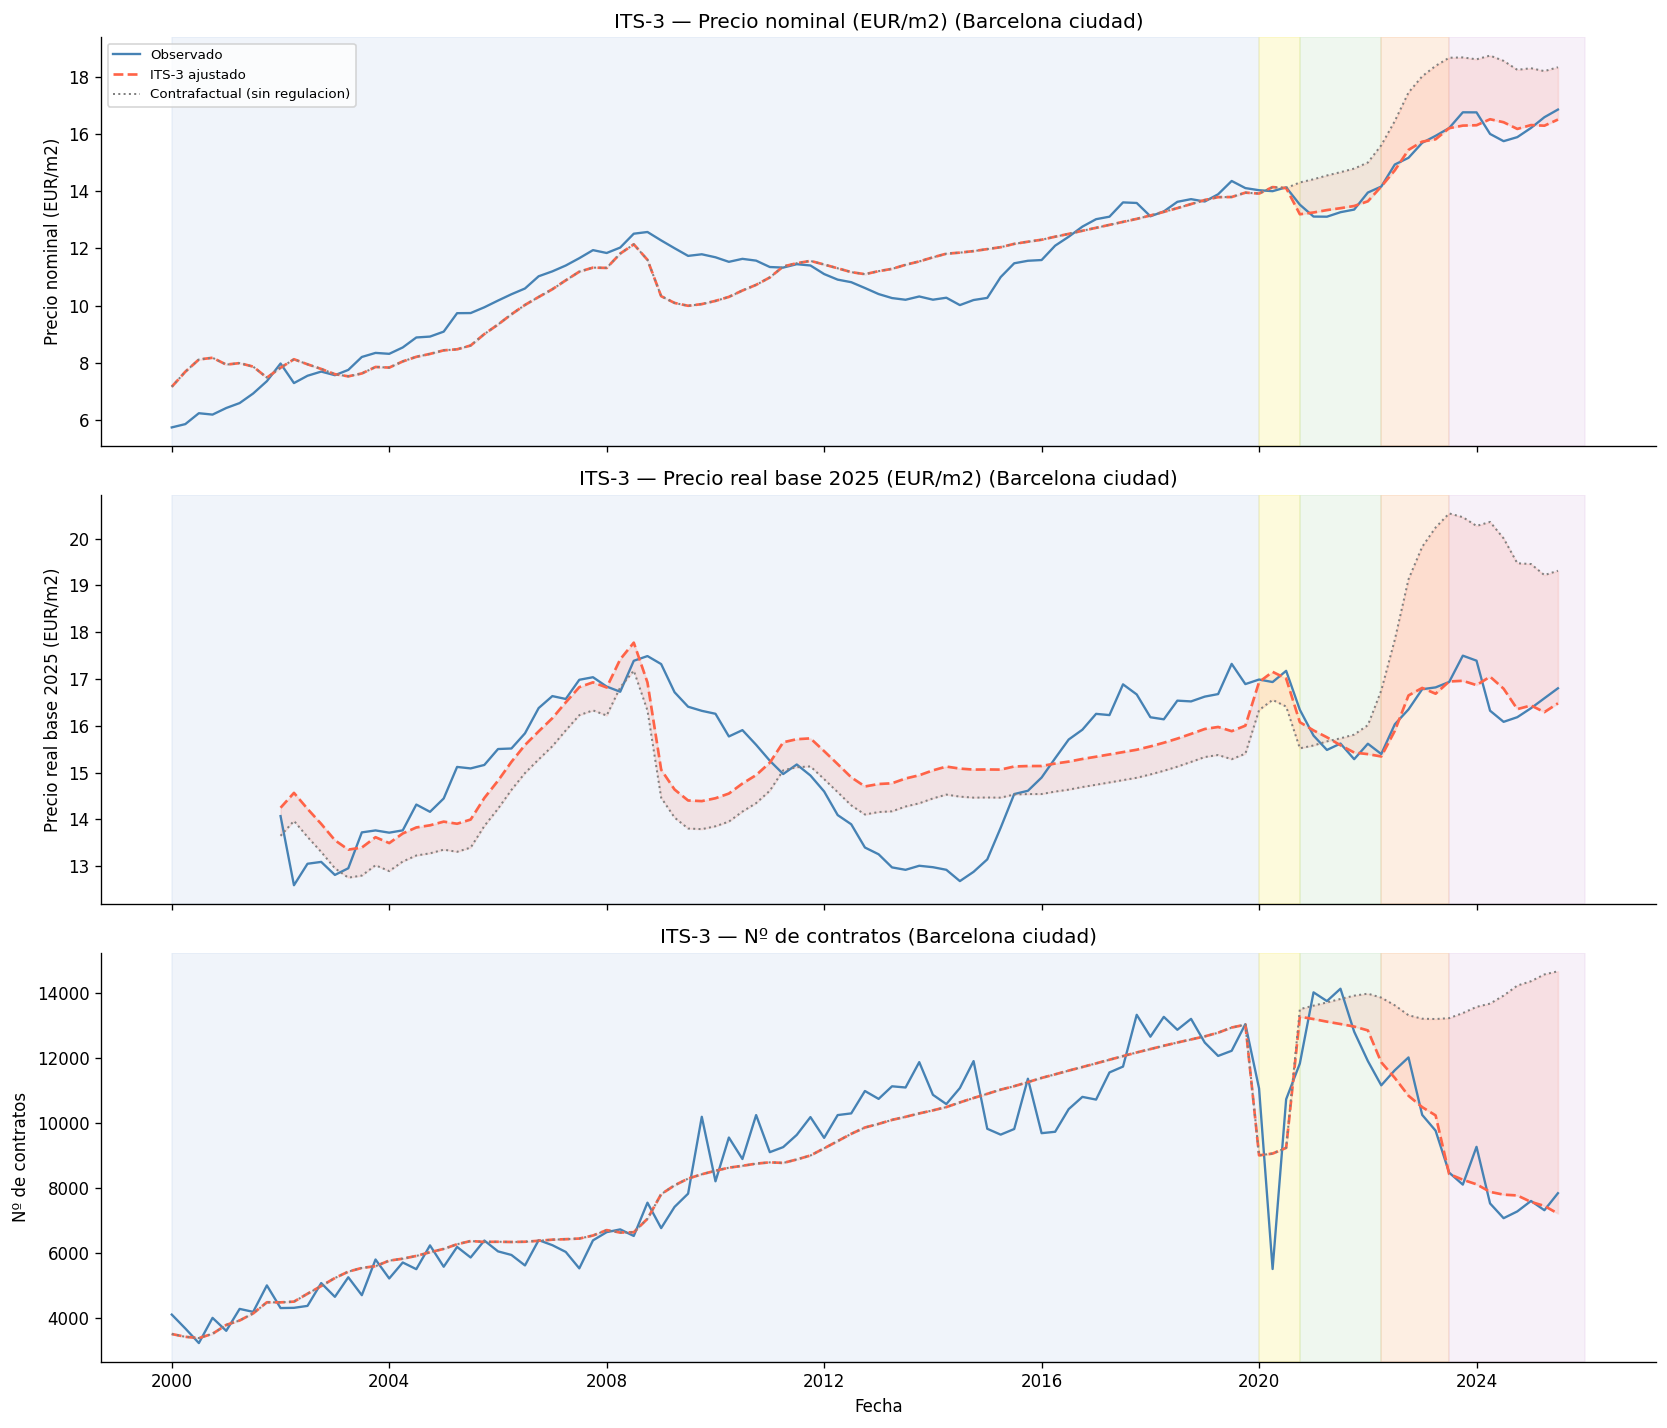
\includegraphics[width=\linewidth]{figures/fig07_its3_city.png}
  \caption{ITS-3 ciudad para las tres métricas. Azul = observado; rojo discontinuo
    = ITS-3 ajustado; gris punteado = contrafactual (tendencia pre-intervención).
    La brecha azul/gris mide el efecto acumulado de la regulación.}
  \label{fig:its3_city}
\end{figure}

\subsubsection{Heterogeneidad geográfica del ITS-3}

La Figura~\ref{fig:its3_dist} muestra el ajuste ITS-3 por los 10 distritos para el
precio nominal. Destaca la mayor amplitud de la brecha observado-contrafactual en
distritos centrales (Gràcia, Eixample, Ciutat Vella).

\begin{figure}[H]
  \centering
  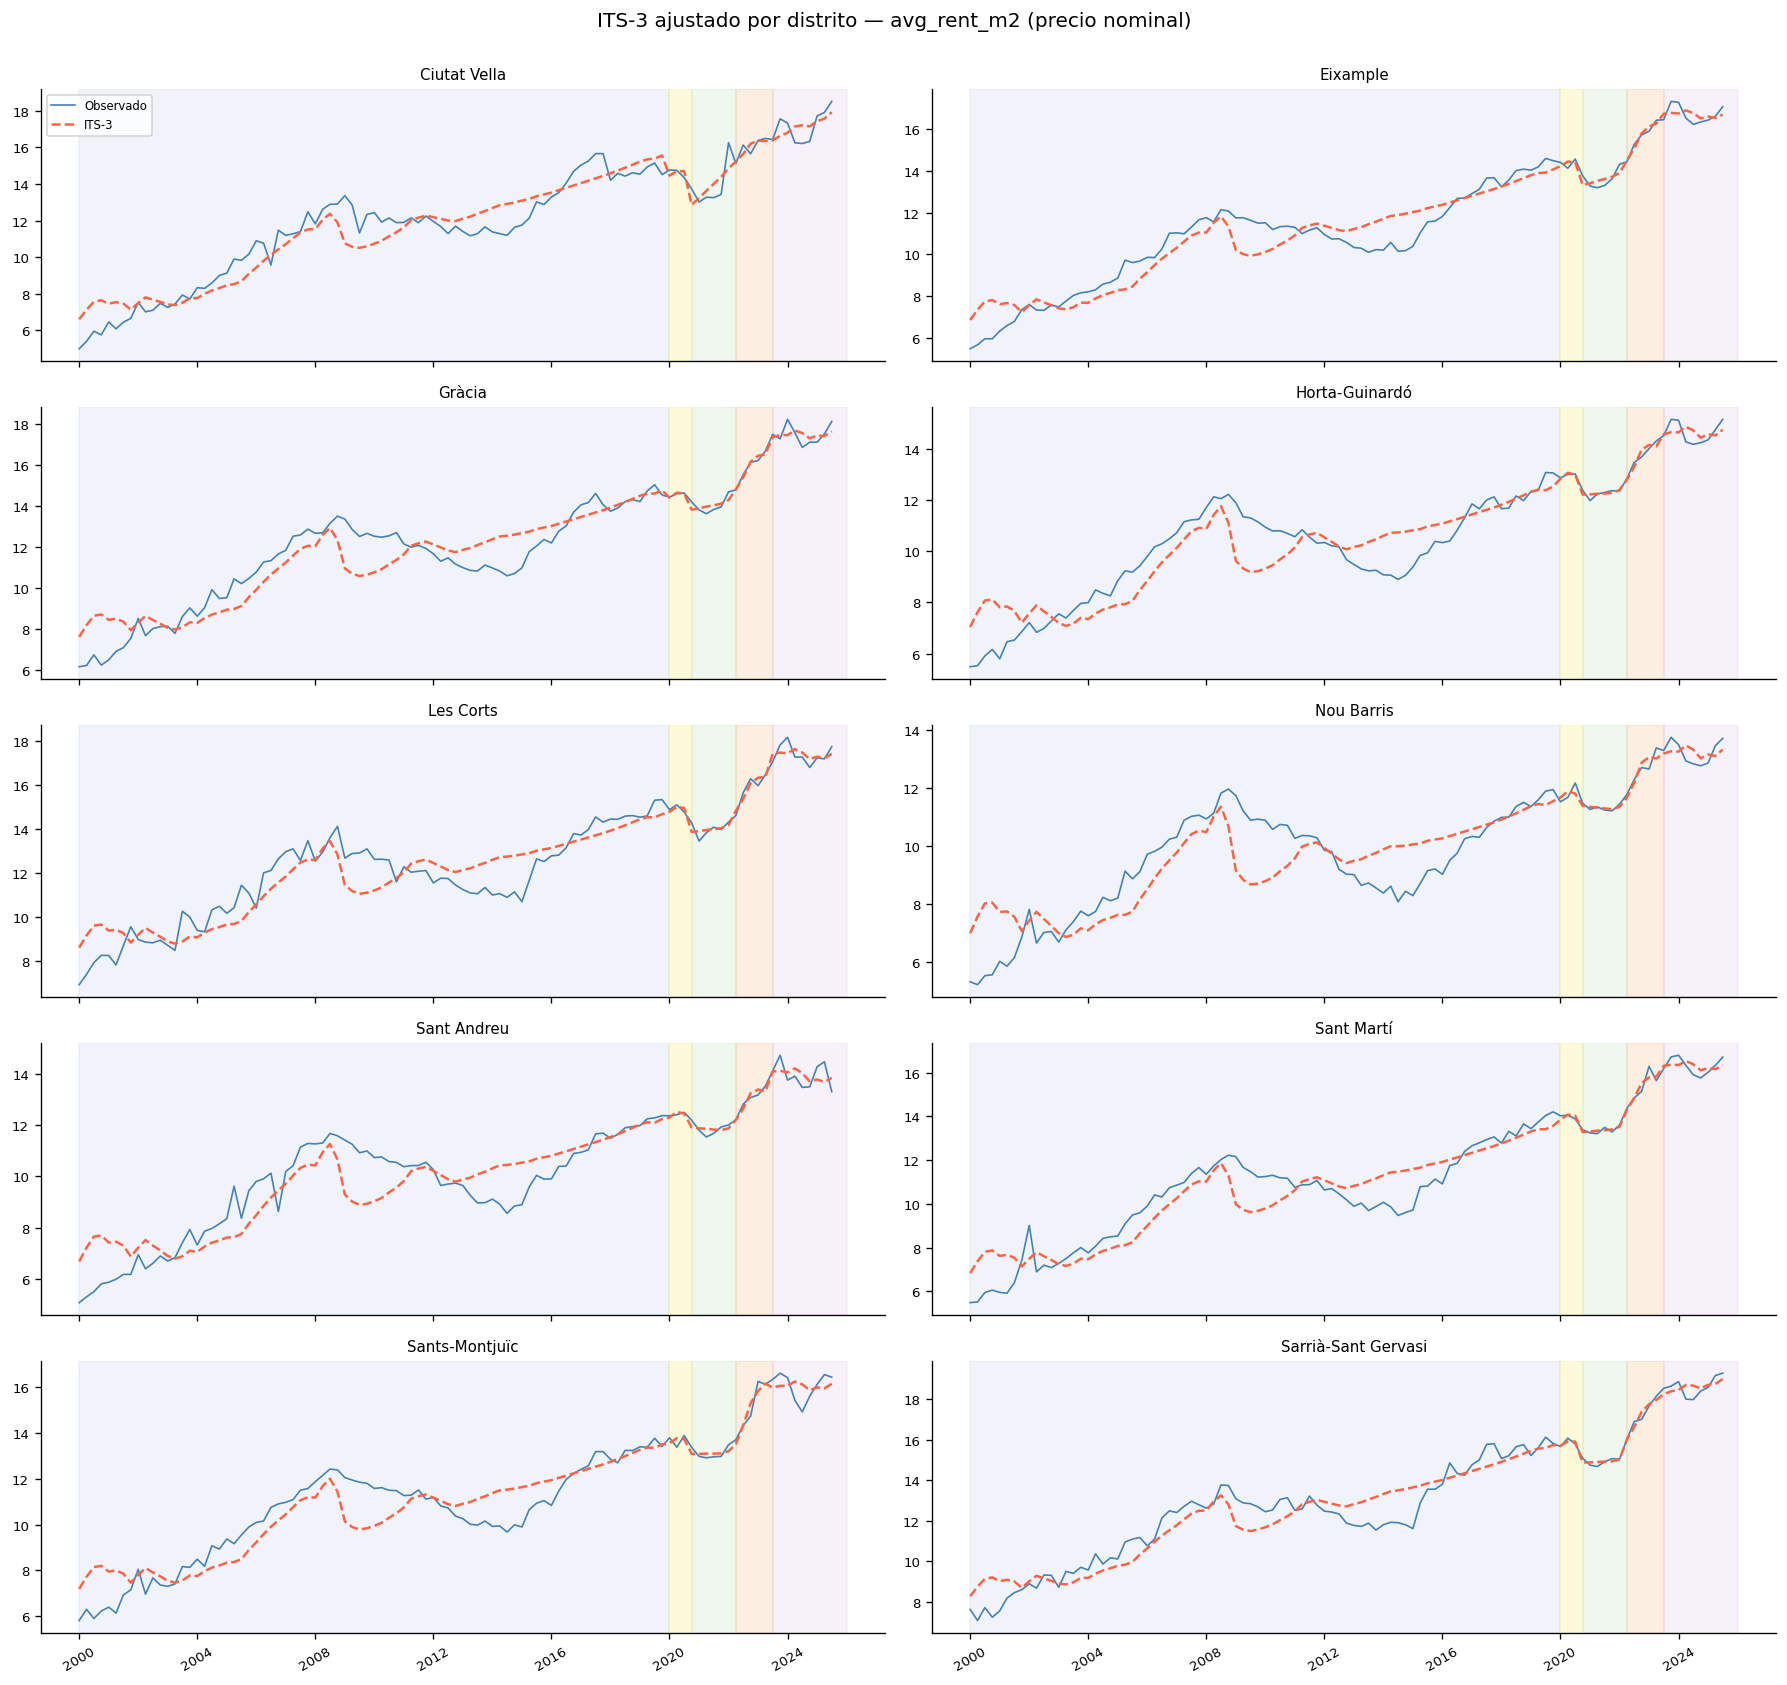
\includegraphics[width=\linewidth]{figures/fig10_its3_districts.png}
  \caption{ITS-3 ajustado (rojo) vs.\ observado (azul) por distrito, precio nominal.
    Las bandas coloreadas son los períodos regulatorios. La heterogeneidad geográfica
    es considerable: la brecha es hasta 3 veces mayor en Gràcia que en Nou Barris.}
  \label{fig:its3_dist}
\end{figure}

La Figura~\ref{fig:heatmap} muestra el heatmap del level shift $D_{ley12}$ por
distrito y métrica.

\begin{figure}[H]
  \centering
  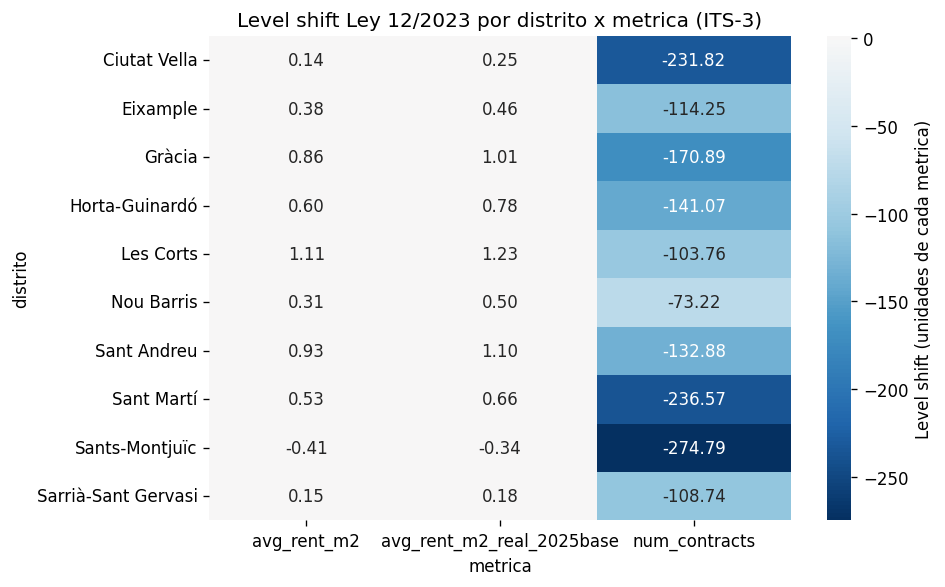
\includegraphics[width=0.88\linewidth]{figures/fig10b_its3_heatmap.png}
  \caption{Level shift $\hat{\beta}_{D_{ley12}}$ (ITS-3) por distrito $\times$
    métrica. Rojo = efecto positivo en precio; azul = contracción en contratos.
    La divergencia precio-volumen es el patrón dominante en todos los distritos.}
  \label{fig:heatmap}
\end{figure}

\subsubsection{Proyecciones condicionales}

La Figura~\ref{fig:projection} muestra las proyecciones a 8 trimestres bajo dos
escenarios de Euríbor con intervalos de confianza al 90\,\%.

\begin{figure}[H]
  \centering
  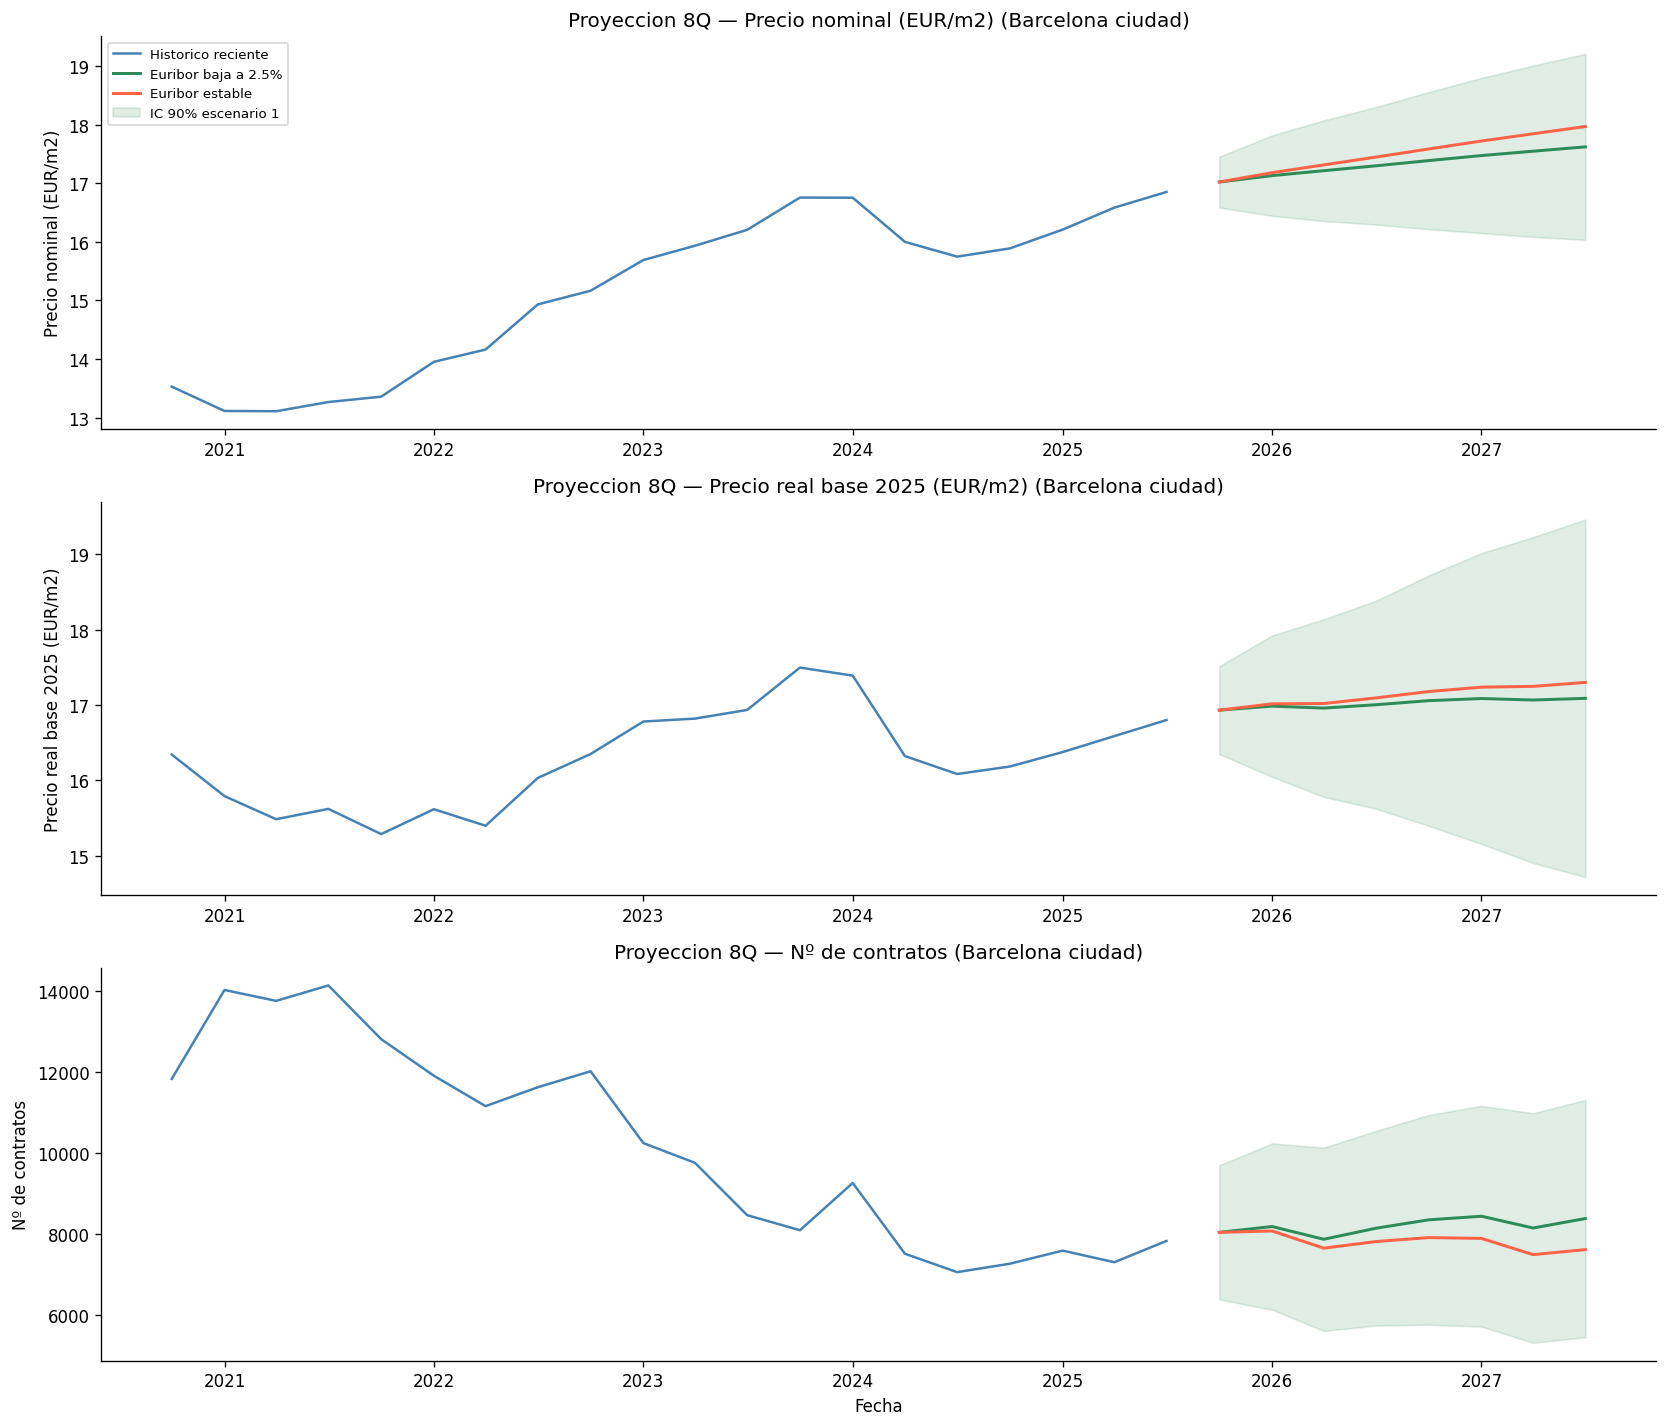
\includegraphics[width=\linewidth]{figures/fig08_projection.png}
  \caption{Proyección condicional (SARIMAX reentrenado sobre serie completa). Verde:
    Euríbor baja a 2.5\,\% en 8 trimestres; rojo: Euríbor estable a 2.12\,\%.
    Banda: IC 90\,\% (escenario verde). Filas: precio nominal, precio real, contratos.}
  \label{fig:projection}
\end{figure}

% ===========================================================
\section{Discusión}
\label{sec:discusion}

\subsection{La paradoja precio-volumen bajo la Ley 12/2023}

El hallazgo central del análisis es la divergencia simultánea entre
$\hat{\beta}_{D_{ley12}}^{(n)}{=}{-}1.588$ en contratos ($p{=}0.007$) y
$\hat{\beta}_{D_{ley12}}^{(r)}{=}{+}0.495$ \euro/m$^2$ en precio real
($p{=}0.034$). Este patrón contradice la lectura simplista de que ``la regulación
no sirvió para nada'': sí redujo el volumen, pero el precio del stock observable subió.

La explicación más parsimonios es el \textbf{efecto composición}: los propietarios
más sensibles al precio (viviendas de menor calidad y precio) abandonaron el mercado
habitual al no poder actualizar renta, mientras los que permanecieron son los de
mayor calidad. El índice $\texttt{avg\_rent\_m2}$ captura la media ponderada del
stock \textit{observable}, que en 2024--2025 es progresivamente más premium.
\citet{diamond2019rent} documentan un mecanismo análogo en San Francisco: $-15\,\%$
de oferta regulada con recomposición hacia usos de mayor valor.

\subsection{El efecto de sustitución no observable}

El dataset solo cubre contratos de larga duración. El crecimiento exponencial de
contratos de temporada ($\leq$11 meses, exentos) en 2023--2025 --- estimado en más
del $40\,\%$ interanual por portales inmobiliarios --- no está capturado, lo que
implica una sobreestimación del efecto regulatorio sobre el volumen si parte de la
demanda simplemente migró de categoría contractual.

\subsection{El canal Euríbor en contexto histórico}

El coeficiente positivo del Euríbor en el ITS nominal ($+0.654$, $p{<}.001$) es
contraintuitivo: el Euríbor alto se asocia a precios más elevados. La explicación es
histórica: en la muestra 2000--2025, los períodos de tipos altos (2005--2008) coinciden
con la bonanza económica cuando el alquiler subía aceleradamente. El estimador OLS en
niveles recoge esta correlación espuria. En el modelo de panel M3, donde la
identificación es \textit{within}-barrio, el coeficiente es correctamente negativo
($-0.076$, $p{<}.001$).

\subsection{Heterogeneidad geográfica y política pública}

La variación de $\hat{\beta}_{D_{ley12}}^{(r)}$ entre distritos --- de $+1.01$
\euro/m$^2$ en Gràcia a $\approx 0$ en Nou Barris --- implica que una política
uniforme por toda Barcelona actúa de forma cualitativamente distinta según el submercado.
Una zonificación más fina (a nivel barrio en lugar de zona tensionada única) podría
reducir la heterogeneidad del efecto.

\subsection{Limitaciones de identificación}

La limitación estructural más relevante es la ausencia de un grupo de control válido:
todos los barrios de Barcelona están bajo el mismo régimen en cada período. El diseño
ITS asume que la tendencia pre-intervención habría continuado \textit{ceteris paribus},
supuesto que puede violarse si otros shocks no observados coinciden con las fechas de
intervención. Los resultados deben interpretarse como \textbf{asociaciones parciales
robustamente estimadas} con HAC, no como efectos causales en sentido estricto.

% ===========================================================
\section{Conclusiones y Líneas Abiertas}
\label{sec:conclusiones}

Presentamos cuatro conclusiones principales:

\begin{enumerate}[leftmargin=*,label=\textbf{C\arabic*.}]

\item \textbf{Efectos diferenciados por ciclo regulatorio.} La Ley~11/2020 produce
un level shift significativo de $-1.11$~\euro/m$^2$ en precio nominal ($p{=}0.007$),
sin efecto en precio real. La derogación TC tiene el impacto más claro en precio real
($-0.558$~\euro/m$^2$, $p{=}0.003$). La Ley~12/2023 contrae contratos
($-1.588$/trim., $p{=}0.007$) pero no contiene el precio real; la evidencia es
inconsistente con el objetivo declarado de asequibilidad.

\item \textbf{El SARIMAX supera los baselines en precio nominal para distritos densos}
(MAPE $2.8$--$3.5\,\%$ vs.\ $6$--$8\,\%$ del naïve), pero el naïve domina en volumen
de contratos. Esto tiene implicaciones prácticas: el método óptimo depende de la
variable a pronosticar.

\item \textbf{La heterogeneidad geográfica es sustancial.} Una política uniforme
produce efectos de magnitud hasta 10$\times$ mayor en Gràcia que en Nou Barris;
la zonificación actual es insuficiente para capturar esta variabilidad.

\item \textbf{La divergencia precio-volumen es la firma del efecto composición.}
La regulación no destruyó demanda ni redujo el precio del stock observable; desplazó
la oferta hacia segmentos no regulados, elevando el precio medio de lo que queda en
el mercado habitual.

\end{enumerate}

\textbf{Líneas abiertas:} \textit{(a)}~Incorporar datos de contratos de temporada
para cuantificar el efecto de sustitución. \textit{(b)}~DiD con municipios de la
RMB como grupo de control. \textit{(c)}~VECM para estimar la elasticidad precio-oferta
en cada régimen. \textit{(d)}~Nowcasting de tensión con datos del Catastro en tiempo
real. \textit{(e)}~Análisis de bienestar para cuantificar el cambio de surplus entre
inquilinos y propietarios.

% ===========================================================
\section*{Agradecimientos}

Los autores agradecen al Ajuntament de Barcelona la disponibilidad pública de los
datos de contratos de alquiler y al equipo docente del Máster de La Salle --
Universitat Ramon Llull su orientación metodológica.

% ── REFERENCIAS ──────────────────────────────────────────────────────────────
\bibliographystyle{apalike}
\begin{thebibliography}{99}

\bibitem[Angrist y Pischke, 2009]{angrist2009mostly}
Angrist, J.~D. y Pischke, J.-S. (2009).
\textit{Mostly Harmless Econometrics}.
Princeton University Press.

\bibitem[Arnott, 1995]{arnott1995rent}
Arnott, R. (1995).
Time for revisionism on rent control?
\textit{J.\ Economic Perspectives}, 9(1):99--120.

\bibitem[Baltagi, 2021]{baltagi2021econometric}
Baltagi, B.~H. (2021).
\textit{Econometric Analysis of Panel Data} (6.ª ed.).
Springer.

\bibitem[Bergmeir et~al., 2018]{bergmeir2018note}
Bergmeir, C., Hyndman, R.~J.\ y Koo, B. (2018).
A note on the validity of cross-validation for evaluating autoregressive time
series prediction.
\textit{Computational Statistics \& Data Analysis}, 120:70--83.

\bibitem[Bosch y Costa, 2021]{bosch2021ley11}
Bosch, J.\ y Costa, A. (2021).
Efectes de la Llei 11/2020 sobre el mercat de lloguer a Catalunya.
\textit{Papers -- Regió Metropolitana de Barcelona}, 63:12--25.

\bibitem[Box et~al., 2015]{box2015timeseries}
Box, G.~E.~P., Jenkins, G.~M., Reinsel, G.~C.\ y Ljung, G.~M. (2015).
\textit{Time Series Analysis: Forecasting and Control} (5.ª ed.).
Wiley.

\bibitem[Diamond et~al., 2019]{diamond2019rent}
Diamond, R., McQuade, T.\ y Qian, F. (2019).
The effects of rent control expansion on tenants, landlords, and inequality.
\textit{American Economic Review}, 109(9):3365--3394.

\bibitem[García-Montalvo y Raya, 2018]{garcia2018housing}
García-Montalvo, J.\ y Raya, J.~M. (2018).
Constraints on housing affordability in Spain.
\textit{Estudios sobre la Economía Española}, SERIEs.

\bibitem[Harvey, 1989]{harvey1989forecasting}
Harvey, A.~C. (1989).
\textit{Forecasting, Structural Time Series Models and the Kalman Filter}.
Cambridge University Press.

\bibitem[Hyndman y Athanasopoulos, 2021]{hyndman2021forecasting}
Hyndman, R.~J.\ y Athanasopoulos, G. (2021).
\textit{Forecasting: Principles and Practice} (3.ª ed.).
OTexts.

\bibitem[Kholodilin et~al., 2021]{kholodilin2021rent}
Kholodilin, K.~A., Kohl, S.\ y Pfeiffer, D. (2021).
Does rent control reduce rents? An economic analysis of Berlin's
  \textit{Mietendeckel}.
\textit{DIW Berlin Discussion Paper}, 1927.

\bibitem[Módenes y López-Colás, 2021]{modenes2021alquiler}
Módenes, J.~A.\ y López-Colás, J. (2021).
El alquiler como modo de tenencia emergente en España.
\textit{Scripta Nova}, 25(660):1--22.

\bibitem[Newey y West, 1987]{newey1987hac}
Newey, W.~K.\ y West, K.~D. (1987).
A simple, positive semi-definite, heteroskedasticity and autocorrelation
consistent covariance matrix.
\textit{Econometrica}, 55(3):703--708.

\bibitem[Sims, 2007]{sims2007rent}
Sims, D.~P. (2007).
Out of control: what can we learn from the end of Massachusetts rent control?
\textit{Journal of Urban Economics}, 61(1):129--151.

\bibitem[Wagner et~al., 2002]{wagner2002its}
Wagner, A.~K., Soumerai, S.~B., Zhang, F.\ y Ross-Degnan, D. (2002).
Segmented regression analysis of interrupted time series studies.
\textit{J.\ Clinical Pharmacy and Therapeutics}, 27(4):299--309.

\bibitem[Ajuntament, 2025]{ajuntament2025}
{Ajuntament de Barcelona} (2025).
Portal de Dades Obertes: Contractes de lloguer per districtes i barris.
\url{https://opendata-ajuntament.barcelona.cat}

\end{thebibliography}

% ===========================================================
\appendix

\begin{table}[H]
\caption{Cronología de períodos regulatorios}
\label{tab:periodos_app}
\centering\small
\begin{tabular}{cll}
\toprule
Cód. & Fechas & Descripción \\
\midrule
P1 & 2000Q1--2019Q4 & Mercado libre \\
P2 & 2020Q1--2020Q3 & COVID shock \\
P3 & 2020Q4--2022Q1 & Ley 11/2020 \\
P4 & 2022Q2--2023Q2 & Derogación TC \\
P5 & 2023Q3--hoy    & Ley 12/2023 \\
\bottomrule
\end{tabular}
\end{table}

\begin{table}[H]
\caption{Orden de integración ADF+KPSS por métrica}
\label{tab:stat_orden_app}
\centering\small
\begin{tabular}{lccc}
\toprule
Métrica & I(0) & I(1) & Ambiguo \\
\midrule
Precio nominal   & 0 & 10 & 0 \\
Precio real 2025 & 1 & 8  & 1 \\
N.º contratos    & 0 & 10 & 0 \\
\bottomrule
\end{tabular}
\end{table}

\end{document}
